\documentclass[11pt]{article}
\usepackage[margin=2.0cm]{geometry}
\usepackage{graphicx,amsmath,booktabs,hyperref,float,caption}
\graphicspath{{./}}
\hypersetup{colorlinks=true,linkcolor=blue,urlcolor=blue}
\captionsetup{font=small}
\newcommand{\Ffsr}{0.8784}
\newcommand{\hard}{0.9876}
\newcommand{\hardpct}{1.24}
\newcommand{\KfiftyThree}{0.111}
\newcommand{\vfiftyThree}{0.31}
\newcommand{\FfiftyThree}{0.8625}
\newcommand{\polchiThree}{51}
\newcommand{\polnThree}{67}
\newcommand{\polmeanThree}{+0.2}
\newcommand{\KfiftyFour}{0.123}
\newcommand{\vfiftyFour}{0.73}
\newcommand{\FfiftyFour}{0.8689}
\newcommand{\polchiFour}{32}
\newcommand{\polnFour}{50}
\newcommand{\polmeanFour}{+1.2}
\newcommand{\vherIn}{0.427}
\newcommand{\ngenRadIn}{1840000}
\newcommand{\nchRadIn}{368}
\newcommand{\ngenBornIn}{3605000}
\newcommand{\nchBornIn}{721}
\newcommand{\sigratioIn}{0.93358}
\newcommand{\nselThreeIn}{22855}
\newcommand{\nselBThreeIn}{54660}
\newcommand{\BherThreeIn}{0.7635}
\newcommand{\BherrThreeIn}{0.0063}
\newcommand{\nselFourIn}{18090}
\newcommand{\nselBFourIn}{42438}
\newcommand{\BherFourIn}{0.7793}
\newcommand{\BherrFourIn}{0.0072}
\newcommand{\vherOut}{0.418}
\newcommand{\ngenRadOut}{1905000}
\newcommand{\nchRadOut}{381}
\newcommand{\ngenBornOut}{3535000}
\newcommand{\nchBornOut}{707}
\newcommand{\sigratioOut}{0.93352}
\newcommand{\nselThreeOut}{23518}
\newcommand{\nselBThreeOut}{52718}
\newcommand{\BherThreeOut}{0.7743}
\newcommand{\BherrThreeOut}{0.0064}
\newcommand{\nselFourOut}{10930}
\newcommand{\nselBFourOut}{24260}
\newcommand{\BherFourOut}{0.7830}
\newcommand{\BherrFourOut}{0.0094}
\newcommand{\keptRad}{0.6168}
\newcommand{\keptBorn}{0.6251}
\newcommand{\keptratio}{0.9867}
\newcommand{\keptpct}{1.33}
\newcommand{\sigpreIn}{0.94621}
\newcommand{\expectclos}{-2.56}
\newcommand{\mxmu}{0.963}
\newcommand{\mxsig}{0.045}
\newcommand{\closB}{0.9336}
\newcommand{\closA}{0.9572}
\newcommand{\closdev}{-2.47}
\newcommand{\Fgen}{0.8862}
\newcommand{\mxsoft}{1.7}
\newcommand{\gnocutThree}{0.9028}
\newcommand{\gmeeThree}{0.8079}
\newcommand{\gfullThree}{0.7881}
\newcommand{\gnocutFour}{0.9130}
\newcommand{\gmeeFour}{0.8091}
\newcommand{\gfullFour}{0.8020}
\newcommand{\prodOne}{0.899}
\newcommand{\prodTwo}{0.913}
\newcommand{\prodThree}{0.917}
\newcommand{\gencOne}{0.890}
\newcommand{\gencTwo}{0.913}
\newcommand{\gencThree}{0.921}

\newcommand{\crad}{C_{\rm rad}}

\title{Radiative correction for near-threshold $J/\psi$ electroproduction at CLAS12:\\
GEMC rad/Born Monte Carlo against the analytic \texttt{rc\_factor}\\[4pt]
\large F18 inbending and outbending, M.~Tenorio's selection}
\author{exclurad\_py study, branch \texttt{jpsi-rc-method-comparison}}
\date{27 October 2026, revised 28 October 2026}

\begin{document}
\maketitle

\begin{abstract}
We compute the radiative correction $\crad$ for $ep\to e'p'J/\psi$, $J/\psi\to e^+e^-$, two ways that share
no code path after event generation.
\textbf{Method~1} is the ratio of the reconstructed radiative and Born arms of the GEMC~5.14 campaign
\texttt{prod\_jpsi\_f18in\_20261009}, with M.~Tenorio's selection applied to both.
\textbf{Method~2} is analytic: the ratio $\sigma_{\rm obs}/\sigma_{\rm Born}$ from \texttt{rc\_factor}, times the
pre-vertex radiator, times the decay-lepton radiation $F(K)$. It uses no Born Monte Carlo.
The rad arm differs from the Born arm in three card fields (\texttt{iborn}, \texttt{itarg}, \texttt{idecay}), so
both methods describe the \emph{whole} correction: electron-line radiation, straggling in the target before the vertex,
and decay-lepton radiation.

First, a normalisation fault in the campaign. The generator's \texttt{sigma\_nb} counts events that its own daughter
preset then drops, so every rad/Born ratio built from it is $\keptpct\%$ high. This is corrected throughout (Sec.~2).

With the nominal cuts written into method~2 ($M(ee)>2.95$~GeV, the MX window of M.~Tenorio), method~2 is 4--6\% \emph{above}
method~1. Three terms, each measured separately, account for most of it:
\begin{itemize}
\item the hard part of the pre-vertex radiator, $-\hardpct\%$;
\item the decay-photon cut acting at $k^*\approx\KfiftyThree$~GeV and not at the $M(ee)$ edge (0.143~GeV), because of the
$M(ee)$ and MX resolution, $-1.1$ to $-1.8\%$;
\item the production cut acting at its effective $v_{50}$, $-0.5$ to $-1\%$.
\end{itemize}
Bin migration and acceptance weighting are each below 2\% except in the threshold bin.
With those two effective edges taken from the MC chain, method~2 follows the \emph{shape} of method~1 in every binning of
the four-track sample ($\chi^2$ per cell $\approx1$) and in $W$, $Q^2$ and M.~Tenorio's $W$ bins of the three-track sample.
Method~1 stays 1--2\% lower. That is the detector's response to the radiating leptons; lepton PID alone accounts for
0.4--0.9\% of it.
It fails in one place: $|t|$ built from $e'e^+e^-$. There, decay-lepton radiation moves $t$ and no analytic factor
contains it. For M.~Tenorio's analysis this is a $t$-dependent systematic in any three-track $t$ result.
Inbending and outbending agree ($\chi^2=\polchiThree/\polnThree$ and $\polchiFour/\polnFour$). So at the
$\sim$1\% level, method~1 measures radiation, not acceptance.
In M.~Tenorio's three $W$ bins, method~1 gives $\crad=0.76$--$0.79$, against the analysis note's $0.88\times0.85=0.75$. The note's $0.88$ for the decay agrees with ours.
The note's $0.85$ for the electron line is 5--7\% below the $\prodOne$--$\prodThree$ that \texttt{rc\_factor} gives at the note's MX cut.
\end{abstract}

\tableofcontents
\newpage

%=====================================================================
\section{The two methods}

\paragraph{Method 1, Monte Carlo.} Both arms were generated with the same box, the same model
(\texttt{jpsi.diffrad\_vm\_pdet}) and the same number of events per chunk. Both were simulated with GEMC~5.14
and reconstructed. M.~Tenorio's selection (Sec.~\ref{sec:sel}) is applied identically to both. Per bin:
\begin{equation}
\crad^{(1)} = \frac{N^{\rm rec}_{\rm rad}/N^{\rm gen}_{\rm rad}\cdot\sigma_{\rm rad}}
                   {N^{\rm rec}_{\rm Born}/N^{\rm gen}_{\rm Born}\cdot\sigma_{\rm Born}} ,
\end{equation}
binned in \emph{reconstructed} kinematics. $N^{\rm gen}$ and $\sigma$ come from the chunks actually read:
\begin{itemize}
\item inbending: \nchRadIn{} rad chunks ($\ngenRadIn$ events) and \nchBornIn{} Born chunks ($\ngenBornIn$);
\item outbending: \nchRadOut{} and \nchBornOut{};
\item $\sigma_{\rm rad}/\sigma_{\rm Born}=\sigratioIn$ and $\sigratioOut$ over those chunks.
\end{itemize}
The raw count ratio is the acceptance ratio. It is \emph{not} $\crad$, and it is never quoted as such here.

\paragraph{Method 2, analytic.} For every selected rad event $i$, at its own reconstructed $(Q^2,W^2,t,\phi)$:
\begin{equation}
\eta_i = \eta_{\rm int}(v)\;\eta_{\rm ext}(v)\;F(K), \qquad
\crad^{(2)} = N\Big/\sum_i \eta_i^{-1}.
\end{equation}
\begin{itemize}
\item $\eta_{\rm int}$ is \texttt{rc\_factor} (\texttt{exclurad\_py/core/rc.py}) with $MX^2<m_U^2+v$. The model is the one whose missing
particle is the one the topology misses:
\begin{itemize}
\item \texttt{jpsi.diffrad\_vm} for $e'e^+e^-$: the proton is missing, and $t$ is taken from $e'$ and $J/\psi$;
\item \texttt{jpsi.diffrad\_vm\_pdet} for $e'e^+e^-p'$: the $J/\psi$ is missing, $t$ is taken from $p'$, and $t_{\rm nucl}=t$ is set per event.
\end{itemize}
The two models have identical structure functions.
\item $\eta_{\rm ext}$ is the pre-vertex radiator of the generator (straggling law $y^{bt}$, vertex uniform in the 5~cm cell), in the
peaking approximation: the probability that the beam photon keeps $v$ below the cut.
\item $F(K)$ is the cumulative decay-photon spectrum of \texttt{generator/decay\_rad.py} (Ehlotzky--Mitter, exponentiated) at
$K=(M_{J/\psi}^2-2.95^2)/2M_{J/\psi}=0.143$~GeV, where 2.95~GeV is the lower edge of M.~Tenorio's $M(ee)$ window, 2.95--3.20~GeV: $F=\Ffsr$. This reproduces the $0.88$ of the analysis note.
\end{itemize}
Rad events are distributed as $\sigma_{\rm Born}\,\eta\,{\rm Acc}$, so $\crad^{(2)}$ is the Born- and
acceptance-weighted mean of $\eta$ in the bin. This is exactly what method~1 weights by. We also compute the flat average
(no acceptance) on a grid, to measure the weighting.

Both methods use the same radiative engine, so this is a test of the \emph{method}, not of QED. What differs: method~2 knows two
numbers about the selection, the $v$ cut and the $M(ee)$ edge. Method~1 knows the whole selection and the detector.

%=====================================================================
\section{Monte Carlo sample}
\begin{itemize}
\item \texttt{ifarm:/volatile/clas12/vpk/prod\_jpsi\_f18in\_20261009}, out\_inb and out\_outb of both arms, GEMC~5.14.
Copied to \texttt{/Volumes/wd\_14tb/rc\_method\_jpsi}: 2177 files, every one 5000 events $\times$ 80 floats, identical to
ifarm by sha256 (0 mismatches). The farm fill was still running; this is a fixed snapshot.
\item Card differences between the arms: \texttt{iborn} (0/1), \texttt{itarg} (1/0), \texttt{idecay} (2/1). All three are part of
the correction. The Born arm is the cross section at nominal beam energy, with no straggling and no decay radiation.
\item Vertex: generated $v_z$ is uniform over $-5.5\ldots-0.5$~cm in all four samples (mean $-3.0$, rms 1.44~cm). The
$v_z=0$ defect of the superseded Born vintage is absent.
\item Generator commits: four, all \texttt{-dirty} (7d91bc7, a245229, a2c878d, ff3b63a in Born; a2c878d, ff3b63a, one 8ac2fc0
in rad). The arms are not of one vintage. The generator-level closure (Sec.~\ref{sec:closure}) shows no effect of that at
the 0.2\% level.
\item \textbf{Normalisation.} The generator's \texttt{sigma\_nb} is counted from every event that passed its
accept--reject. The \texttt{iacc=jpsi} preset on the decay daughters ($|p|>1$~GeV, $5$--$40^\circ$) is applied
\emph{afterwards}, and the events that fail it are dropped. In every chunk, accepted $-$ \texttt{cut\_acceptance} $=5000$
written. So $\sigma_{\rm nb}/5000$ overweights each written event, and not equally in the two arms: a hard decay or
production photon leaves a lepton below 1~GeV. The preset keeps $\keptRad$ of rad and $\keptBorn$ of Born.
All $\sigma$ here are therefore $\sigma_{\rm nb}\times$ written/accepted, chunk by chunk. The rad/Born ratio of
the written events is $\sigratioIn$, not $\sigpreIn$: a factor $\keptratio$, or $-\keptpct\%$, on every method-1 number.
The same correction applies to any $n_{\rm rad}/n_{\rm Born}\times\sigma_{\rm rad}/\sigma_{\rm Born}$ built from
\texttt{sigma\_nb} on an \texttt{iacc}$\neq$\texttt{none} campaign. That includes the generated-10M per-bin tables,
shown corrected here ($^*$).
\item F18 outbending ran at two torus settings: $+1.008$ for runs 5423--5476 (25.3\% of the data) and $+1.000$ for
5478--5666 (74.7\%). The simulation has $+1.000$, so the outbending MC represents three quarters of that run period.
\end{itemize}

%=====================================================================
\section{Event selection}\label{sec:sel}
The analysis note of M.~Tenorio, Secs.~3--4, as far as the ntuple carries the variable. The cuts are applied identically to both arms and both topologies:
\begin{itemize}
\item Scattered electron: an identified FT electron ($|{\rm status}|$ 1000--1999, pid 11). The note's FT-face fiducial cut
$8<r<15.75$~cm becomes $2.45^\circ<\theta_e<6.45^\circ$. The ntuple has no FT hit position. On M.~Tenorio's F18in
$e'e^+e^-$ data this window reproduces the $r$ cut event by event for 91\% of events.
\item $\nu>8.1$~GeV.
\item Leptons: pid $\pm11$, $|p|>1.95$~GeV, $e^-$ $|p|<10.6$~GeV. $-8<v_z<4$~cm on the inward-bending lepton.
\item $2.95<M(ee)<3.20$~GeV.
\item $e'e^+e^-$: $\Delta p_z>-2.5$~GeV, and $MX(e'e^+e^-)$ within $\mu\pm4\sigma$, with $\mu=\mxmu$ and $\sigma=\mxsig$~GeV from a
Gaussian fit to the Born MC (the note's rule, applied to our sample). Its upper edge is $v=\vherIn$ (inb) and $\vherOut$ (outb)~GeV$^2$.
\item $e'e^+e^-p'$: proton pid 2212 with $|p|>0.4$~GeV, $-0.7<\Delta p_z<0.5$~GeV, $|MX^2(e'e^+e^-p')|<0.036$~GeV$^2$.
\end{itemize}
\textbf{Not applied}, because the ntuple does not carry them: PCAL energy and fiducial, BDT scores, the triangular cut,
$\chi^2_{\rm PID}$, $\beta$, the $\theta(E)$ cut on two-hit FT clusters, and lepton timing.

Selected events, inbending: $e'e^+e^-$ $\nselThreeIn$ rad / $\nselBThreeIn$ Born; $e'e^+e^-p'$ $\nselFourIn$ / $\nselBFourIn$.
Outbending: $\nselThreeOut$ / $\nselBThreeOut$ and $\nselFourOut$ / $\nselBFourOut$.

Table~\ref{tab:cutvars} gives each cut N$-$1: the survival of the cut with all others applied, rad over Born. The cuts are
strongly correlated \emph{through the decay photon}. Its momentum is missing from $MX(e'e^+e^-)$ and from $\Delta p_z$, so
those cuts remove decay-radiation events before $M(ee)$ sees them. In the three-track sample, $M(ee)$ alone then costs only 1\%,
not 12\%. N$-$1 ratios therefore do not factorise $\crad$, and the decomposition is done on the effective edges
instead (Sec.~\ref{sec:diff}).
\begin{table}[H]\centering\small
\begin{tabular}{lcccc}\toprule
$e'e^+e^-$: cut & rad keeps (inb) & Born keeps (inb) & $r$ inb & $r$ outb \\\midrule
FT theta e & 0.9998 & 1.0000 & 0.9998$\pm$0.0001 & 1.0000$\pm$0.0001 \\
nu $>$ 8.1 & 1.0000 & 1.0000 & 1.0000$\pm$0.0000 & 1.0000$\pm$0.0000 \\
lepton PID & 0.7539 & 0.7609 & 0.9907$\pm$0.0040 & 0.9963$\pm$0.0040 \\
lepton $|$p$|$ & 0.9979 & 0.9981 & 0.9998$\pm$0.0004 & 1.0003$\pm$0.0004 \\
vz & 0.9877 & 0.9889 & 0.9988$\pm$0.0009 & 0.9999$\pm$0.0009 \\
M(ee) & 0.9485 & 0.9567 & 0.9913$\pm$0.0018 & 0.9928$\pm$0.0018 \\
dpz & 0.9347 & 0.9414 & 0.9929$\pm$0.0021 & 0.9921$\pm$0.0021 \\
MX window & 0.9513 & 0.9728 & 0.9779$\pm$0.0017 & 0.9771$\pm$0.0017 \\
\bottomrule\end{tabular}

\medskip

\begin{tabular}{lcccc}\toprule
$e'e^+e^-p'$: cut & rad keeps (inb) & Born keeps (inb) & $r$ inb & $r$ outb \\\midrule
FT theta e & 0.9998 & 1.0000 & 0.9998$\pm$0.0001 & 1.0000$\pm$0.0000 \\
nu $>$ 8.1 & 1.0000 & 1.0000 & 1.0000$\pm$0.0000 & 1.0000$\pm$0.0000 \\
lepton PID & 0.7713 & 0.7761 & 0.9937$\pm$0.0044 & 0.9906$\pm$0.0059 \\
lepton $|$p$|$ & 0.9976 & 0.9979 & 0.9997$\pm$0.0004 & 1.0009$\pm$0.0005 \\
vz & 0.9891 & 0.9885 & 1.0006$\pm$0.0010 & 0.9999$\pm$0.0013 \\
M(ee) & 0.8629 & 0.8878 & 0.9719$\pm$0.0033 & 0.9647$\pm$0.0043 \\
proton & 0.9735 & 0.9718 & 1.0018$\pm$0.0015 & 0.9939$\pm$0.0047 \\
dpz & 0.9903 & 0.9997 & 0.9906$\pm$0.0008 & 0.9967$\pm$0.0006 \\
MX2 total & 0.9841 & 0.9869 & 0.9972$\pm$0.0011 & 0.9963$\pm$0.0015 \\
\bottomrule\end{tabular}

\medskip


\caption{N$-$1 per cut in M.~Tenorio's window ($Q^2$ 0.02--0.12, $W$ 4.15--4.48). $r$ = rad survival / Born survival. A cut that
\texttt{rc\_factor} knows nothing about must give $r=1$ unless radiation acts through it. Lepton PID gives $r=0.991$--$0.996$:
the detector's response to the decay-photon shower next to the lepton.}
\label{tab:cutvars}
\end{table}

%=====================================================================
\section{Generator-level closure}\label{sec:closure}
No detector and no cut. All generated events of both arms are binned in generated kinematics, against \texttt{rc\_factor}
with no cut, evaluated per event on 8000 rad events. With $t$ from the proton, the MC is $\closdev\%$ below the formula
everywhere in $W$, $Q^2$ and $|t|$ (Fig.~\ref{fig:closure}): $\closB$ against $\closA$ integrated.
Two things that \texttt{rc\_factor} does not contain make this up:
\begin{itemize}
\item the energy shift of the pre-vertex radiator, which $\eta_{\rm ext}$ in the peaking approximation leaves out. The campaign's
own itarg$=$1 Born run measures it independently: $\sigma$ falls by $\hardpct\%$ (0.345396 against 0.349740~nb);
\item the generation acceptance on the decay daughters, which removes $\keptpct\%$ more rad than Born events (Sec.~2).
\end{itemize}
Together they predict $\expectclos\%$. \textbf{The engine closes to about 0.1\%.} The factor $\hard$ is applied in method~2
from here on. The daughter acceptance needs no factor: the analysis cut $|p|>1.95$~GeV is tighter, so the events it removes would
fail the analysis cuts anyway.

With $t$ built from the $e^+e^-$ pair, the same closure fails by $-35\%$ to $+20\%$ across $|t|$, while $W$ and
$Q^2$ stay within 1--3\%. Decay-lepton radiation takes momentum out of the pair and moves $t$. Nothing analytic contains
that. It returns in Sec.~\ref{sec:diff}.
\begin{figure}[H]\centering
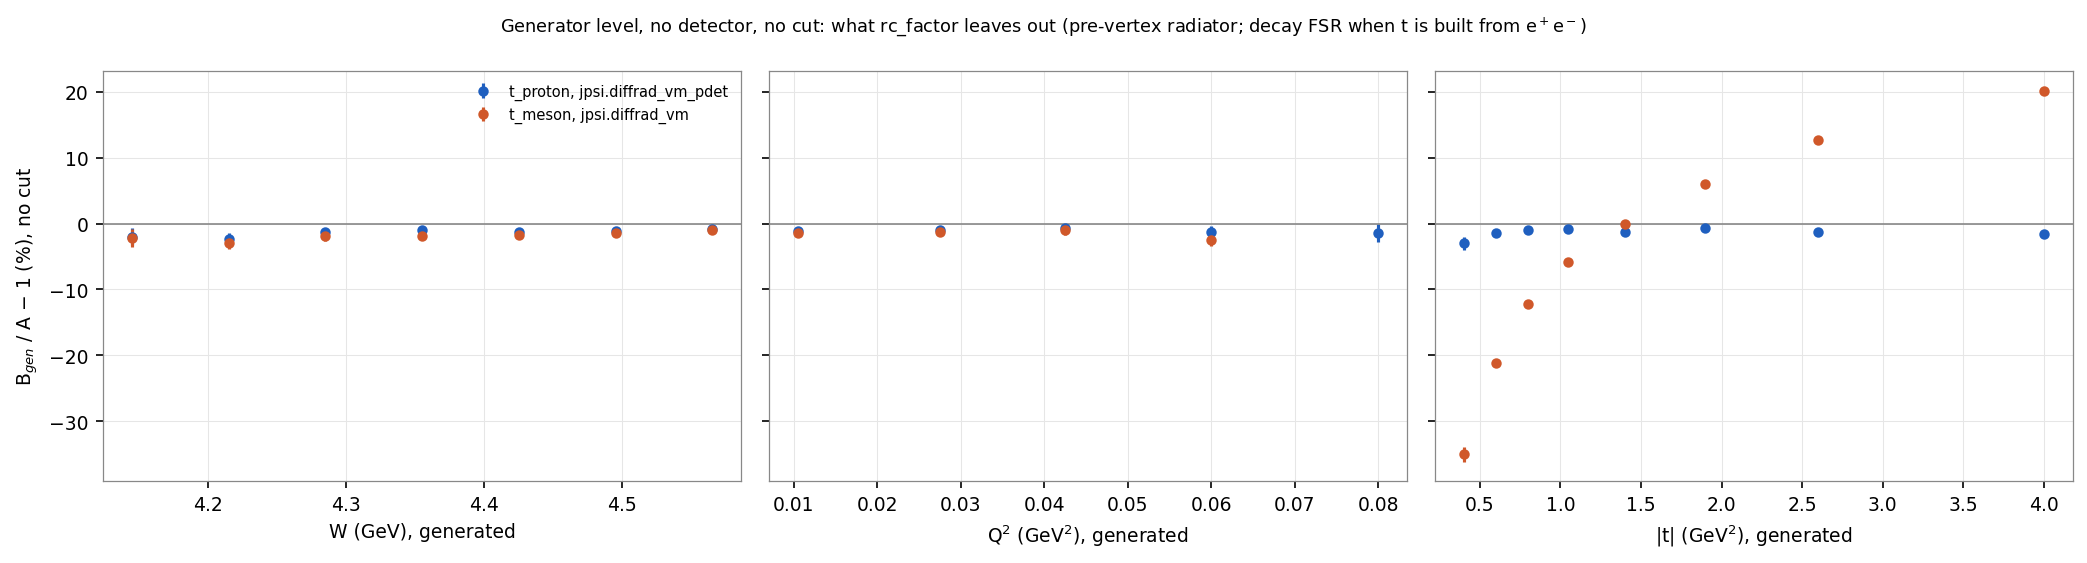
\includegraphics[width=\textwidth]{f7_closure.png}
\caption{Generator level, no cut: generated rad/Born over \texttt{rc\_factor}.}\label{fig:closure}
\end{figure}

The analysis kinematic cuts applied to the \emph{generated} momenta, still with no detector, are shown in Table~\ref{tab:gencuts}.
The generated decay-photon fraction below the $M(ee)$ edge is $\Fgen$, against $F=\Ffsr$ from the formula. This is
\emph{not} the majorant ripple, which lives in the production-photon sampler. Bin by bin, the generated $k^*$ spectrum follows
the formula to 1\% from 1~MeV to 1~GeV. Above $k^*=1$~GeV the generator has 0.0074 of the decays against 0.0159.
Those are exactly the decays whose softer lepton fails the generation preset (Sec.~2). Renormalised over the rest,
$F$ comes out 0.9\% high. The decay generator is correct; the written sample is conditioned on the preset. The MX window removes another
$\mxsoft\%$ of the \emph{soft} decay-photon events, which pass $M(ee)$.
\begin{table}[H]\centering\small
\begin{tabular}{llcccc}\toprule
topology & step & her window & W 4.15--4.29 & W 4.29--4.40 & W 4.40--4.48 \\\midrule
$e'e^+e^-$ & no cut & 0.9150 & 0.8892 & 0.9226 & 0.9250 \\
$e'e^+e^-$ & M(ee) & 0.8188 & 0.7958 & 0.8255 & 0.8279 \\
$e'e^+e^-$ & + dpz & 0.8094 & 0.7867 & 0.8132 & 0.8208 \\
$e'e^+e^-$ & + MX window & 0.7988 & 0.7835 & 0.8031 & 0.8047 \\
$e'e^+e^-$ & MX window only & 0.8187 & 0.8075 & 0.8262 & 0.8189 \\
\midrule
$e'e^+e^-p'$ & no cut & 0.9253 & 0.8983 & 0.9335 & 0.9358 \\
$e'e^+e^-p'$ & M(ee) & 0.8200 & 0.7962 & 0.8269 & 0.8295 \\
$e'e^+e^-p'$ & + dpz & 0.8128 & 0.7944 & 0.8193 & 0.8190 \\
$e'e^+e^-p'$ & + MX2 total & 0.8128 & 0.7944 & 0.8193 & 0.8190 \\
$e'e^+e^-p'$ & dpz only & 0.8504 & 0.8353 & 0.8574 & 0.8538 \\
\bottomrule\end{tabular}

\caption{$\crad$ at generator level with M.~Tenorio's kinematic cuts on generated $e',e^\pm,p'$ (no photons, nominal beam), F18in files.}
\label{tab:gencuts}
\end{table}

%=====================================================================
\section{Results}
\subsection{M.~Tenorio's three $W$ bins}
\begin{table}[H]\centering\footnotesize
\begin{tabular}{llcccccc}\toprule
topology & W (GeV) & method 1 inb & method 1 outb & method 2 nominal & method 2 effective & generated 10M & M.~Tenorio \\\midrule
$e'e^+e^-$ & 4.15--4.29 & 0.767$\pm$0.017 & 0.784$\pm$0.017 & 0.800 & 0.772 & 0.902 & 0.75 \\
$e'e^+e^-$ & 4.29--4.40 & 0.774$\pm$0.011 & 0.783$\pm$0.011 & 0.812 & 0.780 & 0.925 & 0.75 \\
$e'e^+e^-$ & 4.40--4.48 & 0.776$\pm$0.009 & 0.786$\pm$0.009 & 0.816 & 0.783 & 0.933 & 0.75 \\
\midrule
$e'e^+e^-p'$ & 4.15--4.29 & 0.771$\pm$0.020 & 0.738$\pm$0.035 & 0.808 & 0.775 & 0.902 & 0.75 \\
$e'e^+e^-p'$ & 4.29--4.40 & 0.786$\pm$0.012 & 0.787$\pm$0.016 & 0.826 & 0.787 & 0.925 & 0.75 \\
$e'e^+e^-p'$ & 4.40--4.48 & 0.798$\pm$0.010 & 0.804$\pm$0.013 & 0.834 & 0.793 & 0.933 & 0.75 \\
\bottomrule\end{tabular}

\caption{$\crad$ in M.~Tenorio's bins, $Q^2$ 0.02--0.12. Method~2 is inbending; method~2 has no torus in it.
``Nominal'': the analysis MX edge (three tracks) or no $v$ cut (four tracks; the four-track selection has no $MX(e'p)$ cut), $F$ at
$M(ee)=2.95$. ``Effective'': the edges where the analysis chain actually cuts (Sec.~\ref{sec:diff}). ``Generated 10M$^*$'': the
Launch generator's generator-level numbers (generation acceptance only), with the normalisation correction of Sec.~2.}
\label{tab:mariana}
\end{table}
\begin{figure}[H]\centering
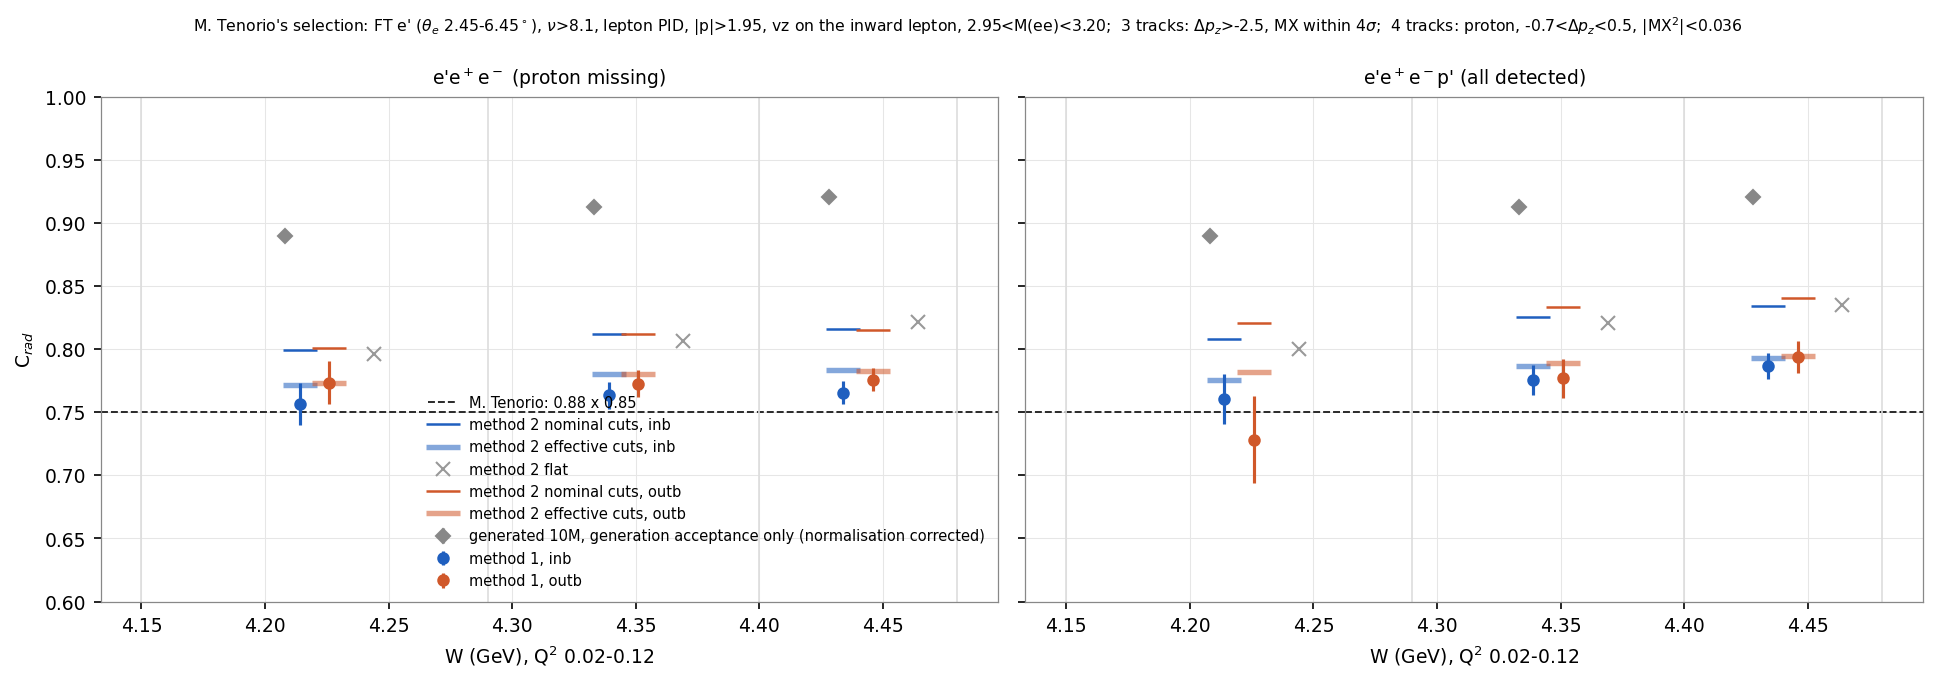
\includegraphics[width=\textwidth]{f3_mariana.png}
\caption{M.~Tenorio's three $W$ bins, both topologies and polarities.}
\end{figure}

\subsection{One variable at a time}
\begin{figure}[H]\centering
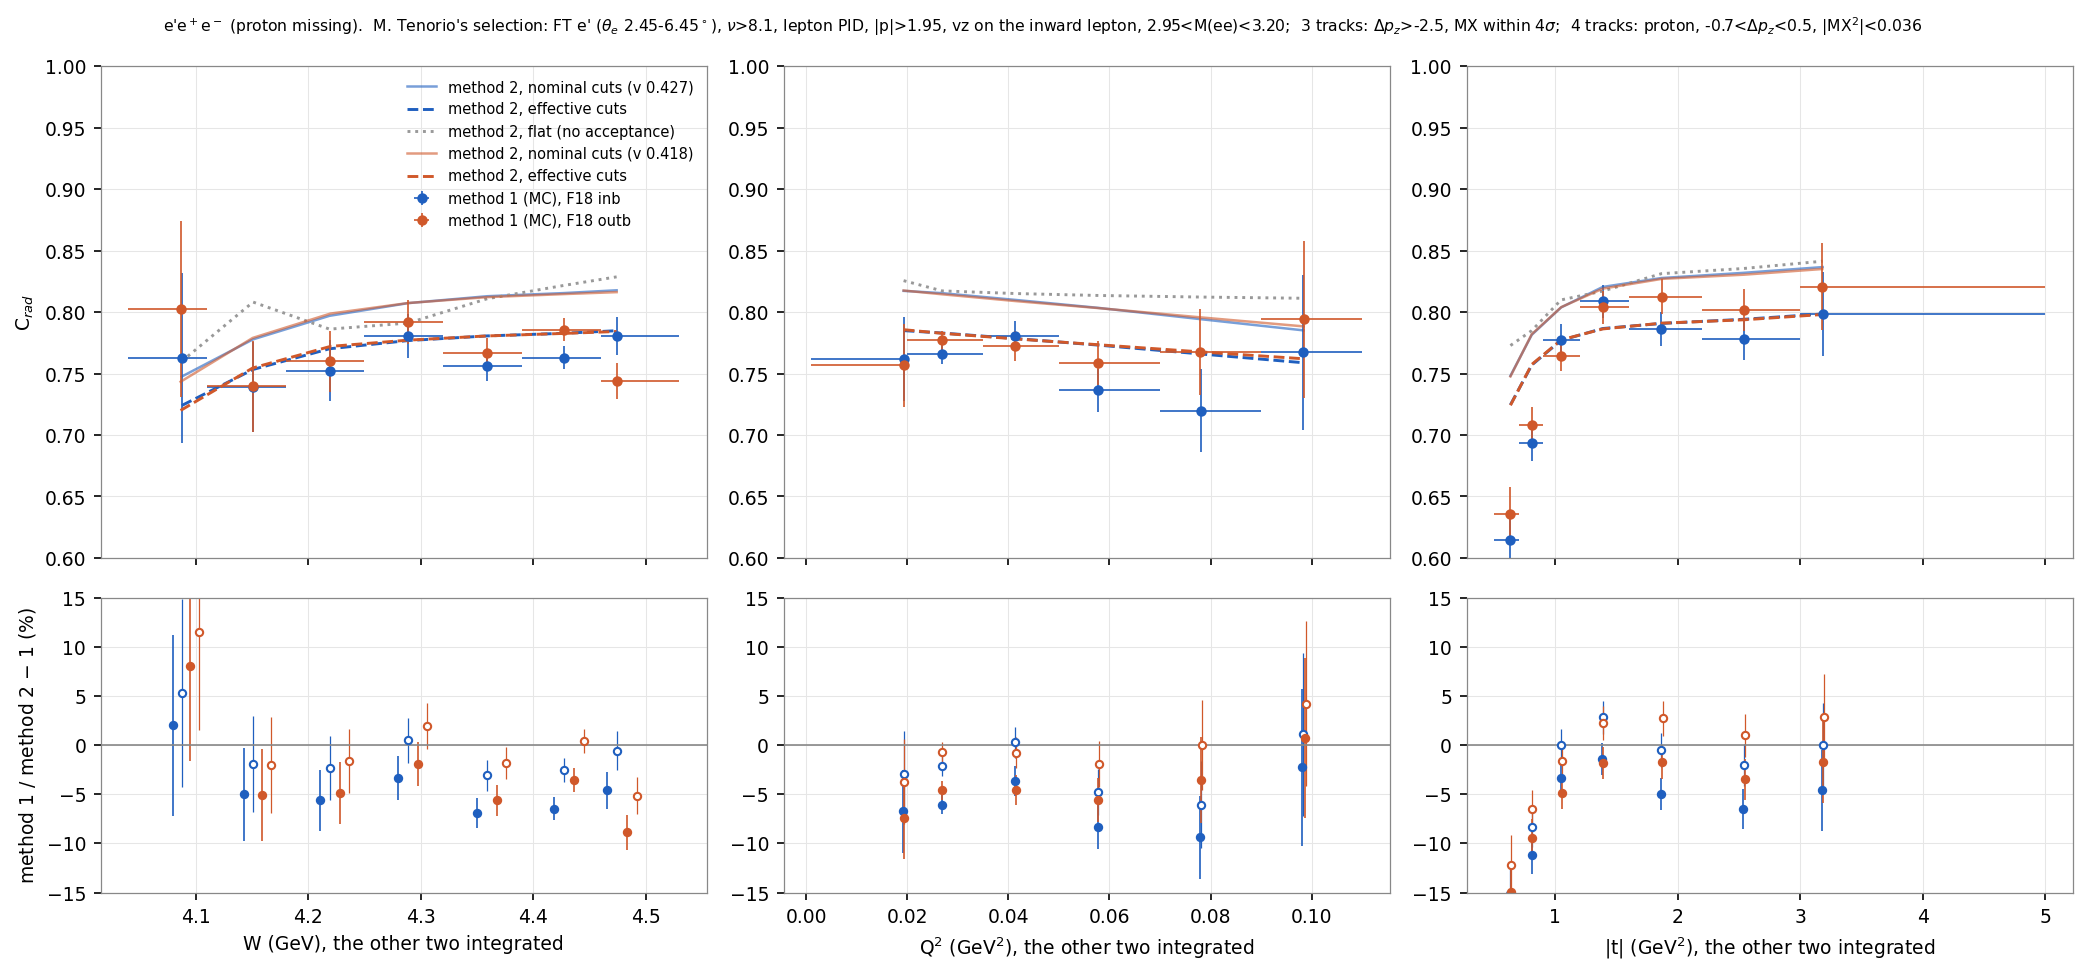
\includegraphics[width=\textwidth]{f1_1d_3trk.png}
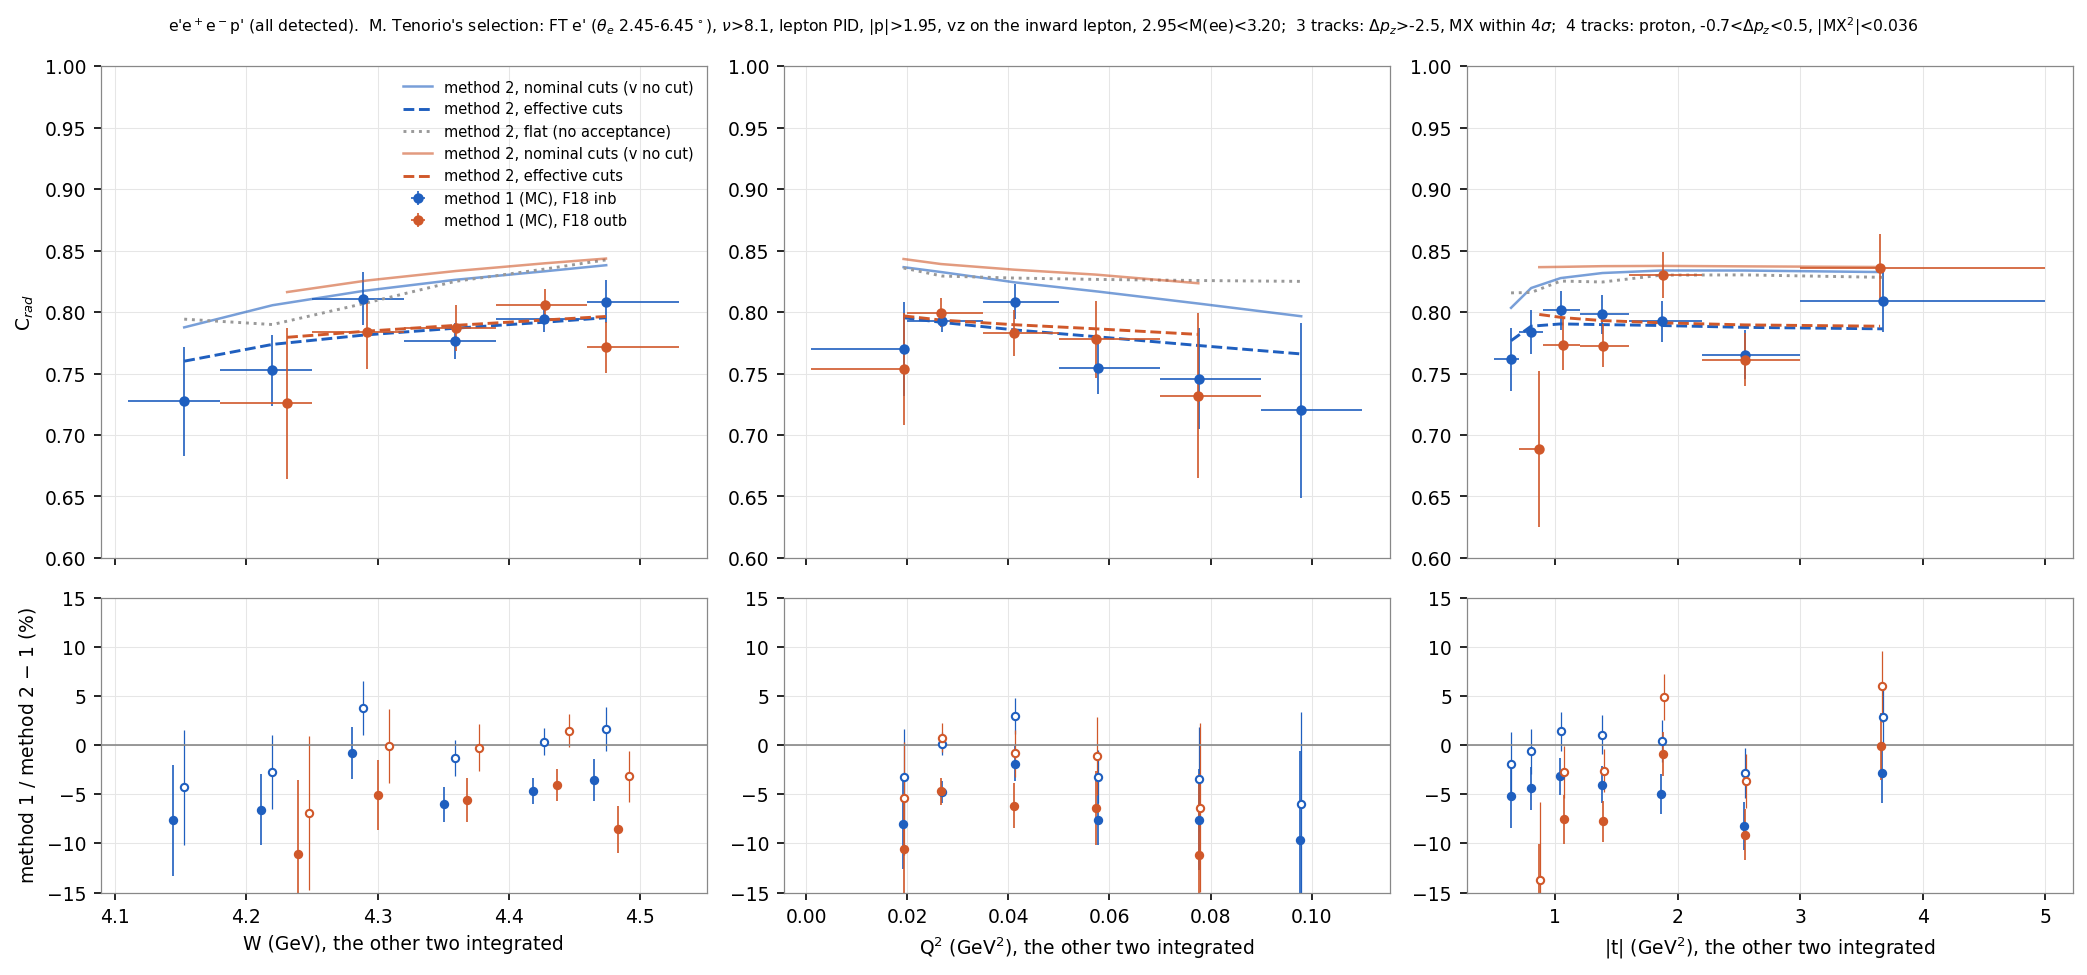
\includegraphics[width=\textwidth]{f1_1d_4trk.png}
\caption{$\crad$ against $W$, $Q^2$, $|t|$, the other two integrated. Solid lines: method~2 at nominal cuts. Dashed lines:
method~2 at effective cuts. Lower panels: method 1/method 2 $-1$, with nominal (filled) and effective (open) cuts.}
\end{figure}

\subsection{The $(W,|t|)$ maps at three $Q^2$}
The brief's $Q^2$ slices (0.02--0.05, 0.05--0.09, 0.09--0.13) do not fit this sample. After the FT cut, 90\% of the events lie
below $Q^2=0.056$ and 1\% above 0.09, so the third slice would be empty. The slices are therefore tertiles of the selected
sample inside the analysis range: 0.02--0.027, 0.027--0.038, 0.038--0.12. The $W$ and $|t|$ edges are quartiles, $4\times4$ per slice.
Most cells carry 4--8\% statistical errors. These maps are a coarse first pass: they test the methods against each
other, and they cannot resolve a structure of a few percent inside a slice.
\begin{figure}[H]\centering
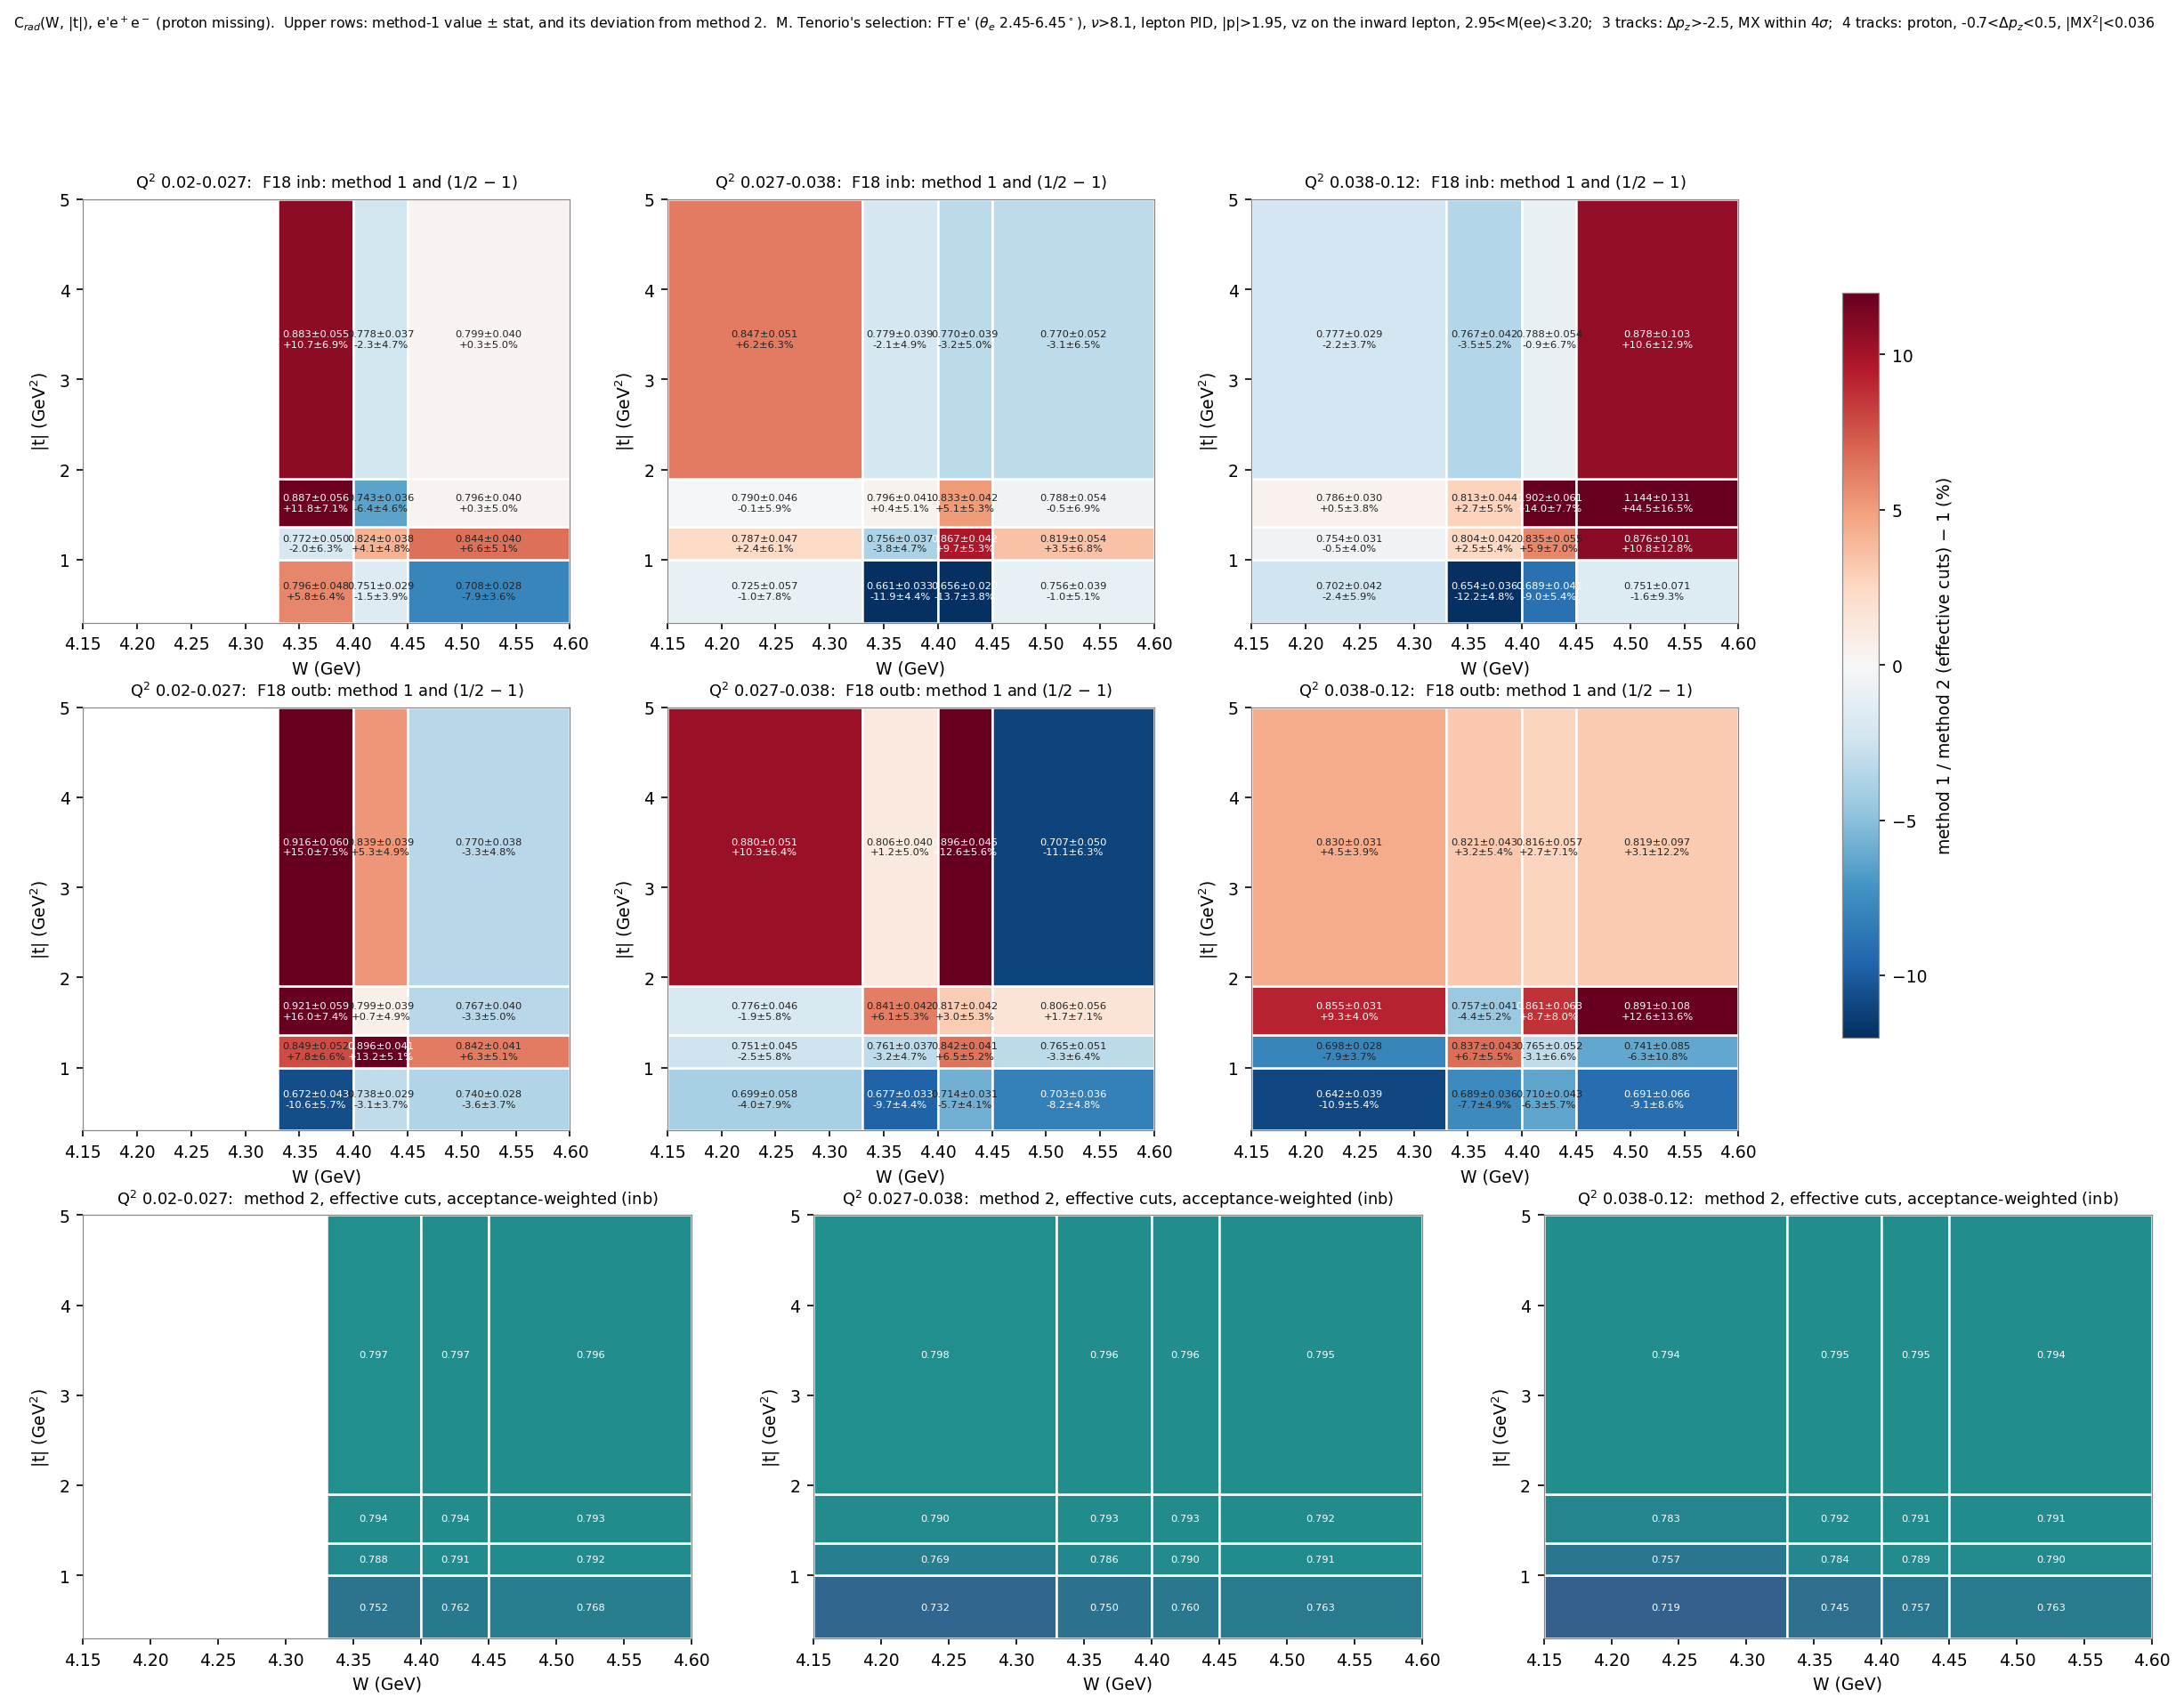
\includegraphics[width=\textwidth]{f2_maps_3trk.png}
\caption{$e'e^+e^-$: method~1 $\pm$ stat and its deviation from method~2 (effective cuts), inb and outb; method~2 in the
bottom row.}
\end{figure}
\begin{figure}[H]\centering
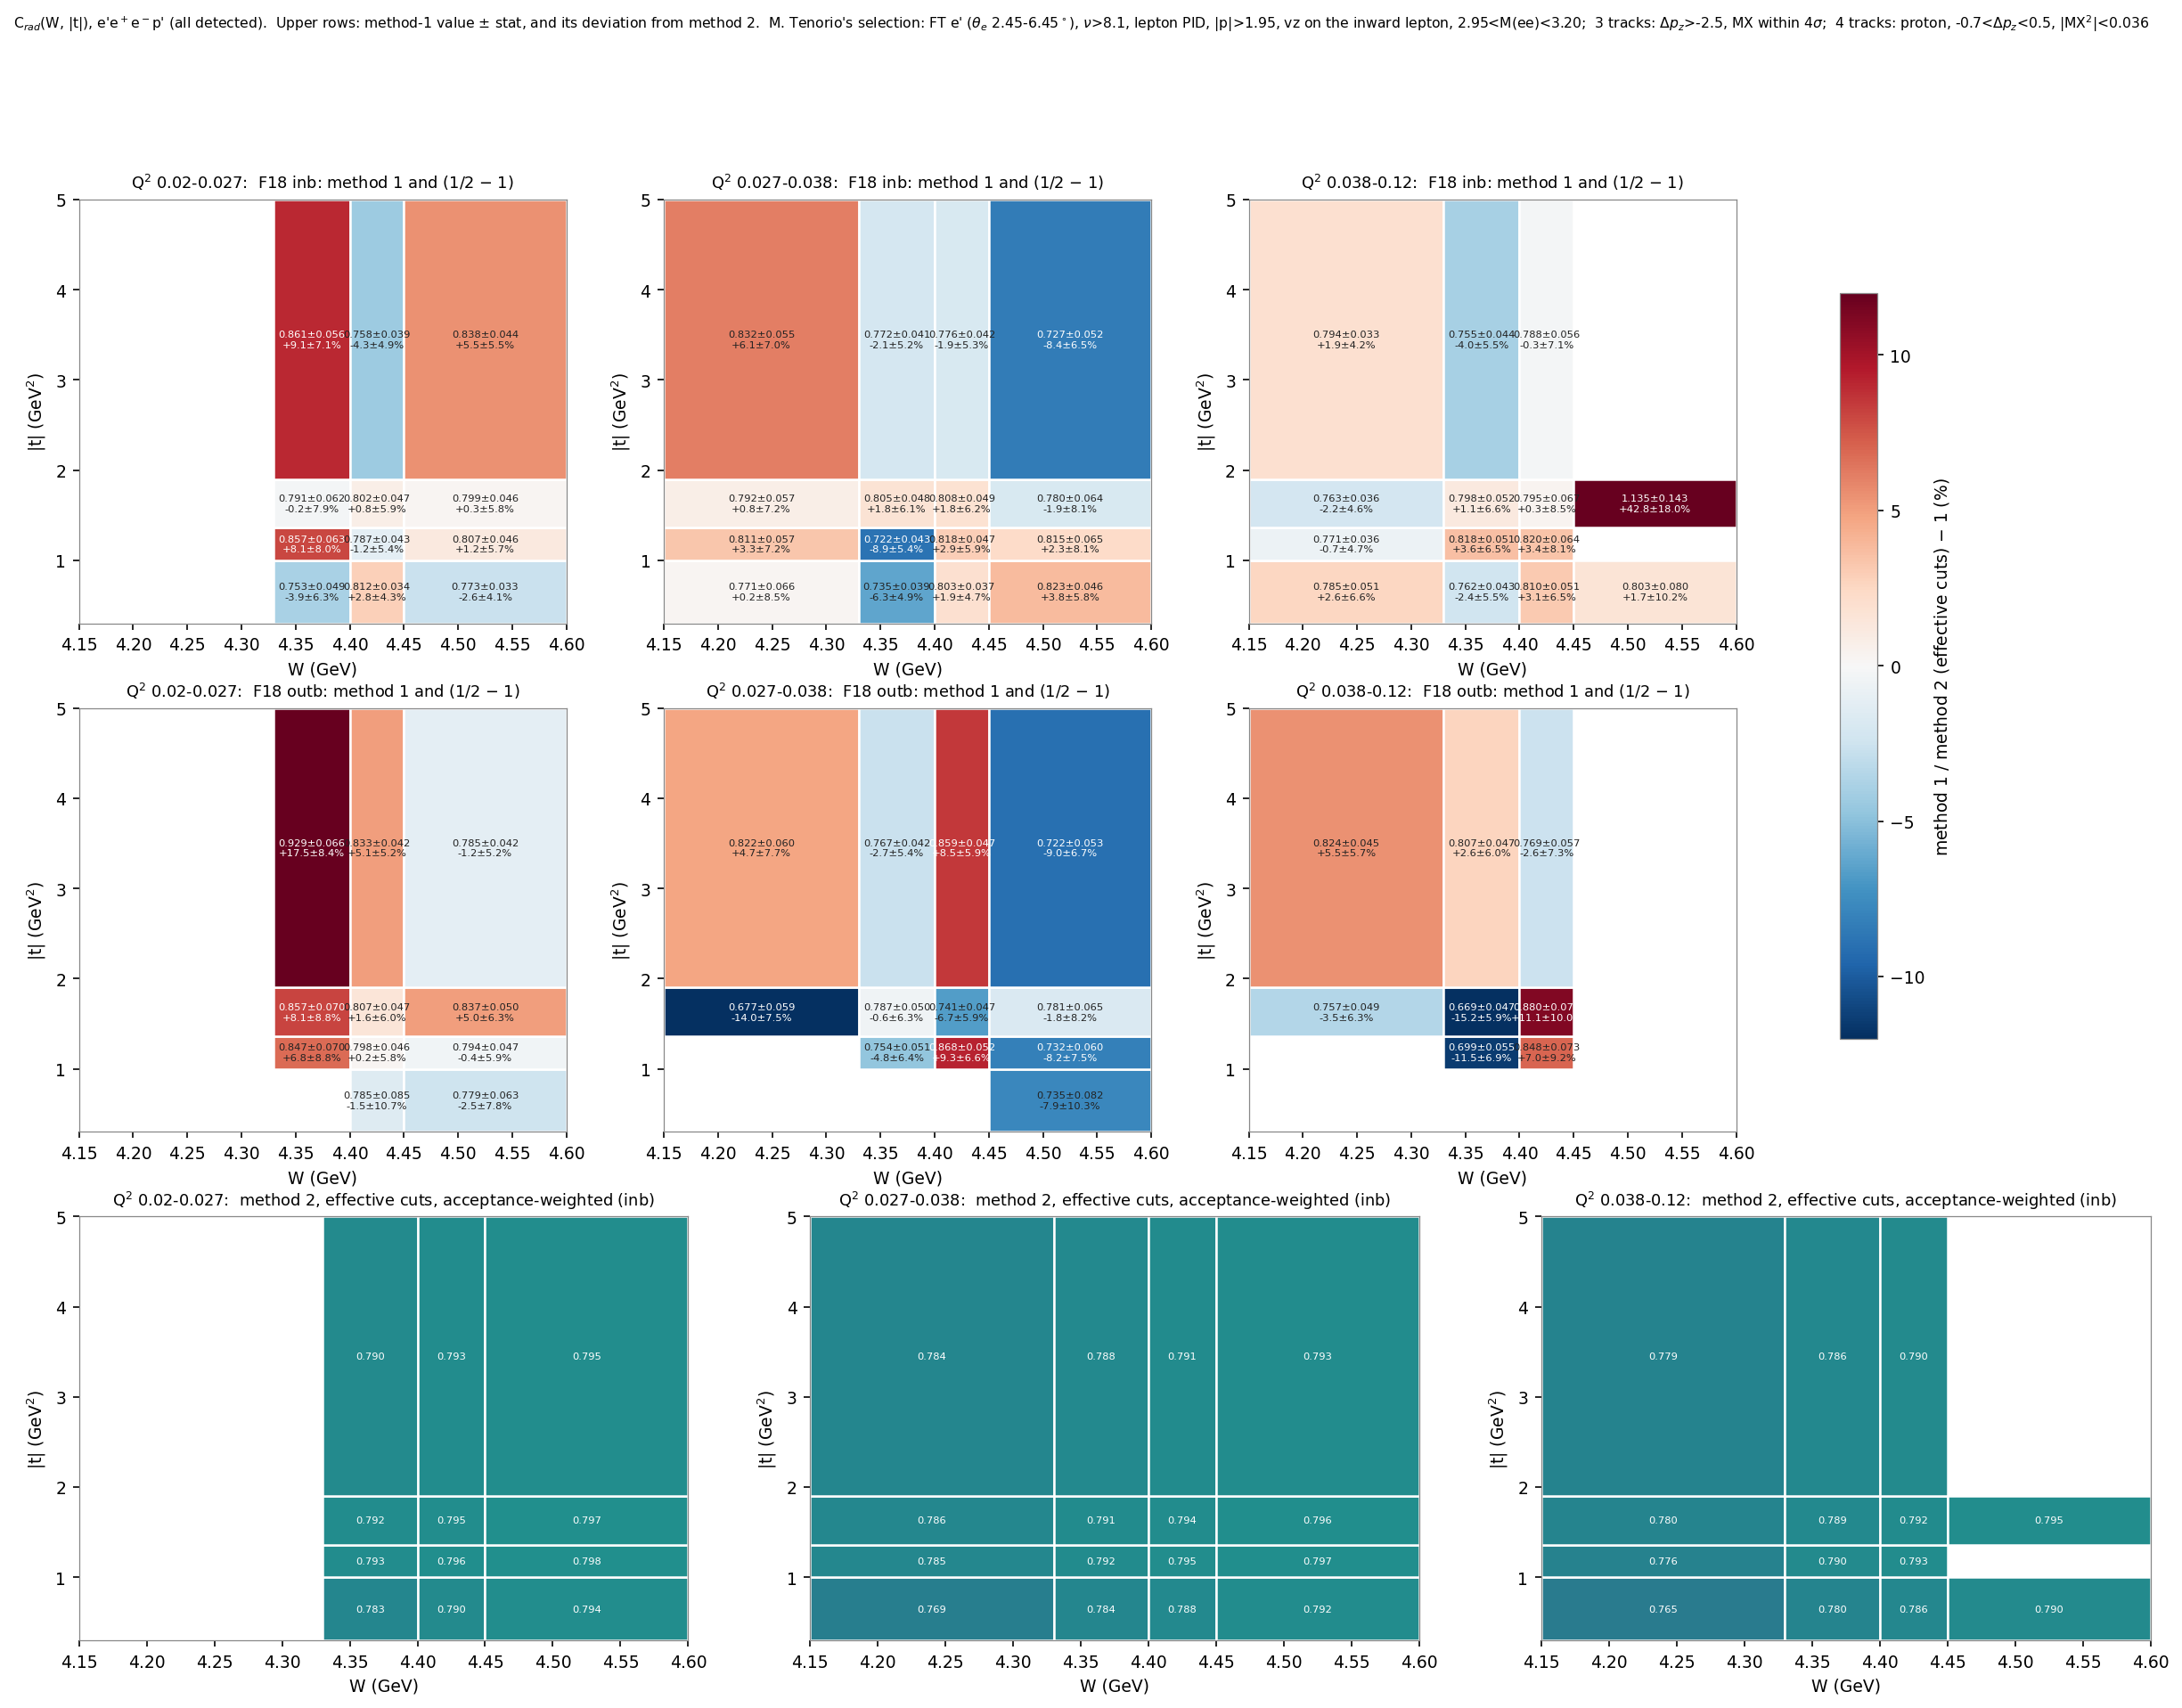
\includegraphics[width=\textwidth]{f2_maps_4trk.png}
\caption{As above, $e'e^+e^-p'$.}
\end{figure}

%=====================================================================
\section{$\crad$ tables for the cross section}\label{sec:tables}
These are the numbers to apply. Each is method~1:
\[
\crad = \frac{N^{\rm rec}_{\rm rad}/N^{\rm gen}_{\rm rad}\cdot\sigma_{\rm rad}}{N^{\rm rec}_{\rm Born}/N^{\rm gen}_{\rm Born}\cdot\sigma_{\rm Born}},
\]
with M.~Tenorio's selection, the $\sigma$ normalisation of Sec.~2, and statistical errors only. The Born cross section in a bin is
\[
\sigma_{\rm Born} = \frac{Y}{\mathcal{L}\;\varepsilon\;\crad}.
\]
\begin{itemize}
\item \textbf{What $\crad$ contains.} It is the \emph{whole} radiative correction: electron-line radiation, straggling before
the vertex, and decay-lepton radiation, all for that selection including the window $2.95<M(ee)<3.20$~GeV. It
\emph{replaces} the note's $0.88\times0.85$; it is not to be multiplied by either factor.
\item \textbf{The efficiency $\varepsilon$ must be a Born efficiency}: Born MC, or M.~Tenorio's own MC without radiation. A radiative
MC efficiency already contains part of $\crad$.
\item \textbf{Hard bins against effective windows.} The analysis yields are counted in the hard $W$ bins (Table~\ref{tab:hardW}), so those
are the factors for the yields. The effective windows (Table~\ref{tab:eff}) are given for completeness; they agree with the hard
bins within errors.
\item \textbf{Topology.} Use the table of the topology the yield comes from: $e'e^+e^-$ and $e'e^+e^-p'$ differ by up to
2--3\% in a bin.
\item \textbf{Polarity.} ``F18 combined'' weights each polarity by its charge (Table~1 of the analysis note: 35.0234 inbending, 32.7332
outbending) times the Born acceptance in that bin. That is how the summed F18 yield of the analysis mixes them. For a yield from one polarity,
use that column. The two agree everywhere within errors (Sec.~\ref{sec:pol}).
\item \textbf{Scope.} F18 at 10.6~GeV only. Spring~2018 (10.6~GeV, other conditions) and Spring~2019 (10.2~GeV) are not
simulated. The outbending MC is at torus $+1.000$. The analysis PCAL, BDT, $\chi^2_{\rm PID}$ and timing cuts are not applied.
\item \textbf{Three-track $|t|$.} Factors binned in $|t|$ from $e'e^+e^-$ (Appendix) carry the decay-radiation migration of
Sec.~\ref{sec:diff}, by construction, since the MC has it. They are correct for $t$ built that way, and only for that.
\end{itemize}
Conventions in every table:
\begin{itemize}
\item ``---'': fewer than 100 events in an arm.
\item $^\dagger$: one polarity only; the other is below threshold.
\item \textit{Italic}: statistical error above 10\%. That is not a measurement; use a coarser bin.
\end{itemize}
All values are also in \texttt{crad\_tables.csv} (232 rows: topology, binning, bin edges, $\crad$ and error per polarity
and combined, event counts).

\begin{table}[H]\centering\small
\begin{tabular}{lcccr}\toprule
\multicolumn{5}{l}{$e'e^+e^-$}\\
W (GeV) & inbending & outbending & \textbf{F18 combined} & $n_{\rm rad}$ \\\midrule
4.15--4.29 & 0.757$\pm$0.017 & 0.773$\pm$0.017 & \textbf{0.765$\pm$0.012} & 5935 \\
4.29--4.40 & 0.763$\pm$0.010 & 0.773$\pm$0.010 & \textbf{0.768$\pm$0.007} & 15477 \\
4.40--4.48 & 0.766$\pm$0.009 & 0.776$\pm$0.009 & \textbf{0.770$\pm$0.006} & 20833 \\
\bottomrule\end{tabular}

\medskip

\begin{tabular}{lcccr}\toprule
\multicolumn{5}{l}{$e'e^+e^-p'$}\\
W (GeV) & inbending & outbending & \textbf{F18 combined} & $n_{\rm rad}$ \\\midrule
4.15--4.29 & 0.760$\pm$0.020 & 0.728$\pm$0.034 & \textbf{0.753$\pm$0.017} & 2768 \\
4.29--4.40 & 0.776$\pm$0.012 & 0.777$\pm$0.015 & \textbf{0.776$\pm$0.009} & 9716 \\
4.40--4.48 & 0.787$\pm$0.010 & 0.794$\pm$0.013 & \textbf{0.790$\pm$0.008} & 14086 \\
\bottomrule\end{tabular}

\medskip


\caption{$\crad$ in M.~Tenorio's hard $W$ bins, $Q^2$ 0.02--0.12 (Table~6 of the analysis note). These are the factors for the $W$-dependent yields.}
\label{tab:hardW}
\end{table}
\begin{table}[H]\centering\small
\begin{tabular}{llcccr}\toprule
\multicolumn{6}{l}{$e'e^+e^-$}\\
$Q^2$ (GeV$^2$) & W (GeV) & inbending & outbending & \textbf{F18 combined} & $n_{\rm rad}$ \\\midrule
0.0253--0.0811 & 4.1813--4.2700 & 0.771$\pm$0.022 & 0.791$\pm$0.023 & \textbf{0.780$\pm$0.016} & 3411 \\
0.0126--0.0620 & 4.3205--4.3911 & 0.761$\pm$0.013 & 0.770$\pm$0.013 & \textbf{0.765$\pm$0.009} & 10026 \\
0.0100--0.0548 & 4.4214--4.5000 & 0.766$\pm$0.010 & 0.772$\pm$0.010 & \textbf{0.769$\pm$0.007} & 18636 \\
\bottomrule\end{tabular}

\medskip

\begin{tabular}{llcccr}\toprule
\multicolumn{6}{l}{$e'e^+e^-p'$}\\
$Q^2$ (GeV$^2$) & W (GeV) & inbending & outbending & \textbf{F18 combined} & $n_{\rm rad}$ \\\midrule
0.0286--0.0711 & 4.2019--4.2560 & 0.795$\pm$0.035 & 0.729$\pm$0.064 & \textbf{0.782$\pm$0.031} & 904 \\
0.0182--0.0467 & 4.3203--4.3867 & 0.763$\pm$0.017 & 0.775$\pm$0.022 & \textbf{0.767$\pm$0.013} & 4834 \\
0.0162--0.0433 & 4.4258--4.4874 & 0.786$\pm$0.012 & 0.774$\pm$0.014 & \textbf{0.781$\pm$0.009} & 10622 \\
\bottomrule\end{tabular}

\medskip


\caption{$\crad$ in the effective $(W,Q^2)$ windows of the analysis note: Table~13 for $e'e^+e^-$, Table~17 for $e'e^+e^-p'$.}
\label{tab:eff}
\end{table}
\begin{table}[H]\centering\small
\begin{tabular}{lcccr}\toprule
\multicolumn{5}{l}{$e'e^+e^-$}\\
$Q^2$ (GeV$^2$) & inbending & outbending & \textbf{F18 combined} & $n_{\rm rad}$ \\\midrule
0.02--0.04 & 0.765$\pm$0.008 & 0.777$\pm$0.008 & \textbf{0.771$\pm$0.005} & 29818 \\
0.04--0.06 & 0.766$\pm$0.013 & 0.775$\pm$0.014 & \textbf{0.771$\pm$0.010} & 9393 \\
0.06--0.11 & 0.742$\pm$0.023 & 0.745$\pm$0.023 & \textbf{0.744$\pm$0.016} & 2990 \\
\bottomrule\end{tabular}

\medskip

\begin{tabular}{lcccr}\toprule
\multicolumn{5}{l}{$e'e^+e^-p'$}\\
$Q^2$ (GeV$^2$) & inbending & outbending & \textbf{F18 combined} & $n_{\rm rad}$ \\\midrule
0.02--0.04 & 0.780$\pm$0.009 & 0.786$\pm$0.011 & \textbf{0.782$\pm$0.007} & 19409 \\
0.04--0.06 & 0.788$\pm$0.016 & 0.787$\pm$0.022 & \textbf{0.788$\pm$0.013} & 5572 \\
0.06--0.11 & 0.750$\pm$0.027 & 0.717$\pm$0.040 & \textbf{0.741$\pm$0.022} & 1572 \\
\bottomrule\end{tabular}

\medskip


\caption{$\crad$ in M.~Tenorio's $Q^2$ bins (Table~21 of the analysis note), $W$ 4.15--4.48.}
\label{tab:Q2}
\end{table}
\begin{table}[H]\centering\small
\begin{tabular}{llcccr}\toprule
\multicolumn{6}{l}{$e'e^+e^-$}\\
$Q^2$ (GeV$^2$) & W (GeV) & inbending & outbending & \textbf{F18 combined} & $n_{\rm rad}$ \\\midrule
0.02--0.04 & 4.15--4.29 & 0.791$\pm$0.032 & 0.825$\pm$0.034 & \textbf{0.807$\pm$0.023} & 1757 \\
0.02--0.04 & 4.29--4.40 & 0.768$\pm$0.013 & 0.774$\pm$0.013 & \textbf{0.771$\pm$0.009} & 10074 \\
0.02--0.04 & 4.40--4.48 & 0.761$\pm$0.010 & 0.775$\pm$0.010 & \textbf{0.767$\pm$0.007} & 17987 \\
0.04--0.06 & 4.15--4.29 & 0.766$\pm$0.026 & 0.737$\pm$0.025 & \textbf{0.752$\pm$0.018} & 2493 \\
0.04--0.06 & 4.29--4.40 & 0.748$\pm$0.020 & 0.791$\pm$0.021 & \textbf{0.769$\pm$0.014} & 4096 \\
0.04--0.06 & 4.40--4.48 & 0.793$\pm$0.025 & 0.788$\pm$0.026 & \textbf{0.791$\pm$0.018} & 2804 \\
0.06--0.11 & 4.15--4.29 & 0.709$\pm$0.030 & 0.779$\pm$0.032 & \textbf{0.743$\pm$0.022} & 1641 \\
0.06--0.11 & 4.29--4.40 & 0.777$\pm$0.036 & 0.708$\pm$0.033 & \textbf{0.743$\pm$0.025} & 1307 \\
0.06--0.11 & 4.40--4.48 & --- & --- & \textbf{---} & 42 \\
\bottomrule\end{tabular}

\medskip

\begin{tabular}{llcccr}\toprule
\multicolumn{6}{l}{$e'e^+e^-p'$}\\
$Q^2$ (GeV$^2$) & W (GeV) & inbending & outbending & \textbf{F18 combined} & $n_{\rm rad}$ \\\midrule
0.02--0.04 & 4.15--4.29 & 0.781$\pm$0.037 & 0.740$\pm$0.059 & \textbf{0.771$\pm$0.032} & 854 \\
0.02--0.04 & 4.29--4.40 & 0.776$\pm$0.015 & 0.786$\pm$0.019 & \textbf{0.779$\pm$0.012} & 6405 \\
0.02--0.04 & 4.40--4.48 & 0.782$\pm$0.011 & 0.788$\pm$0.013 & \textbf{0.784$\pm$0.009} & 12150 \\
0.04--0.06 & 4.15--4.29 & 0.769$\pm$0.030 & 0.740$\pm$0.056 & \textbf{0.763$\pm$0.027} & 1155 \\
0.04--0.06 & 4.29--4.40 & 0.779$\pm$0.023 & 0.761$\pm$0.030 & \textbf{0.773$\pm$0.018} & 2504 \\
0.04--0.06 & 4.40--4.48 & 0.818$\pm$0.029 & 0.841$\pm$0.037 & \textbf{0.826$\pm$0.023} & 1913 \\
0.06--0.11 & 4.15--4.29 & 0.728$\pm$0.036 & 0.693$\pm$0.065 & \textbf{0.721$\pm$0.031} & 742 \\
0.06--0.11 & 4.29--4.40 & 0.768$\pm$0.040 & 0.751$\pm$0.053 & \textbf{0.762$\pm$0.032} & 807 \\
0.06--0.11 & 4.40--4.48 & --- & --- & \textbf{---} & 23 \\
\bottomrule\end{tabular}

\medskip


\caption{$\crad$ on the two-dimensional grid of M.~Tenorio's $W$ bins $\times$ $Q^2$ bins. ``---'': fewer than 100 events per arm. The
cell $Q^2$ 0.06--0.11, $W$ 4.40--4.48 is at the beam-energy edge and holds almost no events.}
\label{tab:WQ2}
\end{table}

\subsection{Three dimensions: $W\times Q^2\times|t|$}
Tables~\ref{tab:WQ2t3} and~\ref{tab:WQ2t4} split every cell of Table~\ref{tab:WQ2} into three $|t|$ bins. The $|t|$ edges,
$0.3$--$1.15$--$1.75$--$5.0$~GeV$^2$, are the tertiles (1.141 and 1.749, rounded) of the selected rad events of both
topologies and both polarities inside $W$ 4.15--4.48, $Q^2$ 0.02--0.11. $|t|$ is taken from $e'e^+e^-$ for three tracks and
from $p'$ for four tracks.
\begin{itemize}
\item \textbf{Kinematic limit.} $|t|_{\min}$ depends on $W$ only (it changes by less than 1\% over this $Q^2$ range):
1.09, 0.75, 0.60 and 0.52~GeV$^2$ at $W=4.15$, 4.29, 4.40 and 4.48~GeV. The first $|t|$ bin therefore starts at
$|t|_{\min}$, not at 0.3: in the lowest $W$ bin, 4.15--4.29, $|t|_{\min}$ falls from 1.09 to 0.75 across the bin, so
the first $|t|$ cell holds only its upper part. Those cells are populated but small.
\item \textbf{Four tracks} ($t$ from the proton): nearly flat. Averaged over $W$ and $Q^2$ the three $|t|$ bins give
0.769, 0.775 and 0.793 ($\pm0.010$ each); $\chi^2=40/23$ against one constant (0.780), from a few cells 2--3$\sigma$ off.
\item \textbf{Three tracks} ($t$ from the lepton pair): the first $|t|$ bin is 11\% lower. Averaged, 0.716, 0.801 and
0.802 ($\pm0.008$); $\chi^2=120/23$ against one constant. This is the decay-radiation migration of Sec.~\ref{sec:diff},
contained in these factors by construction.
\item Statistical errors are 1--7\% per cell (F18 combined). For a $t$ slope, use these with that in mind, or the
one-dimensional $|t|$ table of the Appendix, which has 1--2\%.
\end{itemize}
\begin{table}[H]\centering\footnotesize
\begin{tabular}{lllcccr}\toprule
\multicolumn{7}{l}{$e'e^+e^-$}\\
$Q^2$ (GeV$^2$) & W (GeV) & $|t|$ (GeV$^2$) & inbending & outbending & \textbf{F18 combined} & $n_{\rm rad}$ \\\midrule
0.02--0.04 & 4.15--4.29 & 0.30--1.15 & 0.782$\pm$0.066 & 0.741$\pm$0.065 & \textbf{0.763$\pm$0.046} & 388 \\
0.02--0.04 & 4.15--4.29 & 1.15--1.75 & 0.741$\pm$0.048 & 0.800$\pm$0.051 & \textbf{0.769$\pm$0.035} & 689 \\
0.02--0.04 & 4.15--4.29 & 1.75--5.00 & 0.854$\pm$0.057 & 0.911$\pm$0.060 & \textbf{0.881$\pm$0.041} & 680 \\
0.02--0.04 & 4.29--4.40 & 0.30--1.15 & 0.707$\pm$0.020 & 0.701$\pm$0.020 & \textbf{0.704$\pm$0.014} & 3525 \\
0.02--0.04 & 4.29--4.40 & 1.15--1.75 & 0.815$\pm$0.024 & 0.814$\pm$0.024 & \textbf{0.814$\pm$0.017} & 3421 \\
0.02--0.04 & 4.29--4.40 & 1.75--5.00 & 0.794$\pm$0.024 & 0.826$\pm$0.025 & \textbf{0.809$\pm$0.017} & 3128 \\
0.02--0.04 & 4.40--4.48 & 0.30--1.15 & 0.731$\pm$0.014 & 0.733$\pm$0.014 & \textbf{0.732$\pm$0.010} & 7770 \\
0.02--0.04 & 4.40--4.48 & 1.15--1.75 & 0.795$\pm$0.018 & 0.807$\pm$0.019 & \textbf{0.801$\pm$0.013} & 5352 \\
0.02--0.04 & 4.40--4.48 & 1.75--5.00 & 0.775$\pm$0.019 & 0.812$\pm$0.020 & \textbf{0.793$\pm$0.014} & 4865 \\
0.04--0.06 & 4.15--4.29 & 0.30--1.15 & 0.666$\pm$0.052 & 0.591$\pm$0.046 & \textbf{0.629$\pm$0.035} & 438 \\
0.04--0.06 & 4.15--4.29 & 1.15--1.75 & 0.804$\pm$0.042 & 0.792$\pm$0.041 & \textbf{0.798$\pm$0.029} & 1087 \\
0.04--0.06 & 4.15--4.29 & 1.75--5.00 & 0.778$\pm$0.042 & 0.760$\pm$0.042 & \textbf{0.769$\pm$0.030} & 968 \\
0.04--0.06 & 4.29--4.40 & 0.30--1.15 & 0.707$\pm$0.032 & 0.714$\pm$0.031 & \textbf{0.710$\pm$0.022} & 1438 \\
0.04--0.06 & 4.29--4.40 & 1.15--1.75 & 0.753$\pm$0.035 & 0.813$\pm$0.037 & \textbf{0.782$\pm$0.026} & 1344 \\
0.04--0.06 & 4.29--4.40 & 1.75--5.00 & 0.794$\pm$0.038 & 0.869$\pm$0.041 & \textbf{0.830$\pm$0.028} & 1314 \\
0.04--0.06 & 4.40--4.48 & 0.30--1.15 & 0.727$\pm$0.036 & 0.693$\pm$0.035 & \textbf{0.711$\pm$0.025} & 1121 \\
0.04--0.06 & 4.40--4.48 & 1.15--1.75 & 0.907$\pm$0.051 & 0.858$\pm$0.051 & \textbf{0.885$\pm$0.036} & 897 \\
0.04--0.06 & 4.40--4.48 & 1.75--5.00 & 0.777$\pm$0.047 & 0.879$\pm$0.054 & \textbf{0.823$\pm$0.036} & 786 \\
0.06--0.11 & 4.15--4.29 & 0.30--1.15 & \textit{0.634$\pm$0.064} & 0.726$\pm$0.071 & \textbf{0.678$\pm$0.048} & 281 \\
0.06--0.11 & 4.15--4.29 & 1.15--1.75 & 0.741$\pm$0.048 & 0.777$\pm$0.049 & \textbf{0.759$\pm$0.034} & 702 \\
0.06--0.11 & 4.15--4.29 & 1.75--5.00 & 0.712$\pm$0.048 & 0.806$\pm$0.052 & \textbf{0.757$\pm$0.035} & 658 \\
0.06--0.11 & 4.29--4.40 & 0.30--1.15 & 0.726$\pm$0.059 & 0.630$\pm$0.052 & \textbf{0.679$\pm$0.039} & 414 \\
0.06--0.11 & 4.29--4.40 & 1.15--1.75 & 0.781$\pm$0.061 & 0.749$\pm$0.058 & \textbf{0.765$\pm$0.042} & 470 \\
0.06--0.11 & 4.29--4.40 & 1.75--5.00 & 0.829$\pm$0.068 & 0.752$\pm$0.063 & \textbf{0.792$\pm$0.046} & 423 \\
0.06--0.11 & 4.40--4.48 & 0.30--1.15 & --- & --- & \textbf{---} & 21 \\
0.06--0.11 & 4.40--4.48 & 1.15--1.75 & --- & --- & \textbf{---} & 13 \\
0.06--0.11 & 4.40--4.48 & 1.75--5.00 & --- & --- & \textbf{---} & 8 \\
\bottomrule\end{tabular}

\medskip


\caption{$\crad(W,Q^2,|t|)$, $e'e^+e^-$: M.~Tenorio's $W$ and $Q^2$ bins, $|t|$ tertiles.}
\label{tab:WQ2t3}
\end{table}
\begin{table}[H]\centering\footnotesize
\begin{tabular}{lllcccr}\toprule
\multicolumn{7}{l}{$e'e^+e^-p'$}\\
$Q^2$ (GeV$^2$) & W (GeV) & $|t|$ (GeV$^2$) & inbending & outbending & \textbf{F18 combined} & $n_{\rm rad}$ \\\midrule
0.02--0.04 & 4.15--4.29 & 0.30--1.15 & 0.763$\pm$0.074 & --- & \textbf{0.763$\pm$0.074$^\dagger$} & 151 \\
0.02--0.04 & 4.15--4.29 & 1.15--1.75 & 0.765$\pm$0.060 & --- & \textbf{0.765$\pm$0.060$^\dagger$} & 289 \\
0.02--0.04 & 4.15--4.29 & 1.75--5.00 & 0.808$\pm$0.061 & 0.810$\pm$0.076 & \textbf{0.808$\pm$0.048} & 414 \\
0.02--0.04 & 4.29--4.40 & 0.30--1.15 & 0.736$\pm$0.023 & 0.672$\pm$0.058 & \textbf{0.728$\pm$0.021} & 1655 \\
0.02--0.04 & 4.29--4.40 & 1.15--1.75 & 0.810$\pm$0.028 & 0.780$\pm$0.029 & \textbf{0.797$\pm$0.020} & 2217 \\
0.02--0.04 & 4.29--4.40 & 1.75--5.00 & 0.793$\pm$0.026 & 0.813$\pm$0.028 & \textbf{0.802$\pm$0.019} & 2533 \\
0.02--0.04 & 4.40--4.48 & 0.30--1.15 & 0.799$\pm$0.017 & 0.784$\pm$0.028 & \textbf{0.795$\pm$0.014} & 4427 \\
0.02--0.04 & 4.40--4.48 & 1.15--1.75 & 0.773$\pm$0.021 & 0.761$\pm$0.022 & \textbf{0.767$\pm$0.015} & 3600 \\
0.02--0.04 & 4.40--4.48 & 1.75--5.00 & 0.763$\pm$0.020 & 0.816$\pm$0.022 & \textbf{0.787$\pm$0.015} & 4123 \\
0.04--0.06 & 4.15--4.29 & 0.30--1.15 & 0.761$\pm$0.065 & --- & \textbf{0.761$\pm$0.065$^\dagger$} & 195 \\
0.04--0.06 & 4.15--4.29 & 1.15--1.75 & 0.757$\pm$0.049 & --- & \textbf{0.757$\pm$0.049$^\dagger$} & 415 \\
0.04--0.06 & 4.15--4.29 & 1.75--5.00 & 0.786$\pm$0.049 & 0.737$\pm$0.066 & \textbf{0.771$\pm$0.040} & 545 \\
0.04--0.06 & 4.29--4.40 & 0.30--1.15 & 0.785$\pm$0.038 & --- & \textbf{0.785$\pm$0.038$^\dagger$} & 659 \\
0.04--0.06 & 4.29--4.40 & 1.15--1.75 & 0.753$\pm$0.043 & 0.718$\pm$0.044 & \textbf{0.737$\pm$0.031} & 814 \\
0.04--0.06 & 4.29--4.40 & 1.75--5.00 & 0.794$\pm$0.041 & 0.798$\pm$0.043 & \textbf{0.796$\pm$0.030} & 1031 \\
0.04--0.06 & 4.40--4.48 & 0.30--1.15 & 0.772$\pm$0.042 & \textit{0.638$\pm$0.065} & \textbf{0.741$\pm$0.036} & 610 \\
0.04--0.06 & 4.40--4.48 & 1.15--1.75 & 0.873$\pm$0.059 & 0.970$\pm$0.070 & \textbf{0.915$\pm$0.045} & 618 \\
0.04--0.06 & 4.40--4.48 & 1.75--5.00 & 0.835$\pm$0.054 & 0.847$\pm$0.057 & \textbf{0.841$\pm$0.039} & 685 \\
0.06--0.11 & 4.15--4.29 & 0.30--1.15 & \textit{0.635$\pm$0.071} & --- & \textbf{\textit{0.635$\pm$0.071}$^\dagger$} & 108 \\
0.06--0.11 & 4.15--4.29 & 1.15--1.75 & 0.813$\pm$0.062 & --- & \textbf{0.813$\pm$0.062$^\dagger$} & 288 \\
0.06--0.11 & 4.15--4.29 & 1.75--5.00 & 0.696$\pm$0.055 & \textit{0.748$\pm$0.081} & \textbf{0.712$\pm$0.045} & 346 \\
0.06--0.11 & 4.29--4.40 & 0.30--1.15 & 0.781$\pm$0.067 & --- & \textbf{0.781$\pm$0.067$^\dagger$} & 209 \\
0.06--0.11 & 4.29--4.40 & 1.15--1.75 & \textit{0.677$\pm$0.069} & \textit{0.624$\pm$0.069} & \textbf{0.653$\pm$0.049} & 243 \\
0.06--0.11 & 4.29--4.40 & 1.75--5.00 & 0.829$\pm$0.073 & 0.861$\pm$0.082 & \textbf{0.843$\pm$0.054} & 355 \\
0.06--0.11 & 4.40--4.48 & 0.30--1.15 & --- & --- & \textbf{---} & 4 \\
0.06--0.11 & 4.40--4.48 & 1.15--1.75 & --- & --- & \textbf{---} & 7 \\
0.06--0.11 & 4.40--4.48 & 1.75--5.00 & --- & --- & \textbf{---} & 12 \\
\bottomrule\end{tabular}

\medskip


\caption{As Table~\ref{tab:WQ2t3}, $e'e^+e^-p'$.}
\label{tab:WQ2t4}
\end{table}

%=====================================================================
\section{Where the two methods differ, and why}\label{sec:diff}
Fig.~\ref{fig:vdist} is the key plot. Each cut's survival is plotted against the \emph{generated} radiation: production $v$, and the
decay-photon energy $k^*$ in the $J/\psi$ frame. The analysis chain does not cut where its nominal edges are:
\begin{itemize}
\item \textbf{Decay photon.} The 50\% point of the chain is at $K_{50}=\KfiftyThree$~GeV (three tracks) and $\KfiftyFour$~GeV (four
tracks), not at 0.143. The $M(ee)$ resolution moves events with $k^*\approx0.1$ below 2.95. The MX window and $\Delta p_z$
see the missing photon. $F(K_{50})=\FfiftyThree$ and $\FfiftyFour$, against $\Ffsr$.
\item \textbf{Production radiation.} The 50\% point in $v$ is $\vfiftyThree$~GeV$^2$ (three tracks, the analysis MX window at nominal
$\vherIn$) and $\vfiftyFour$~GeV$^2$ (four tracks, set by $\Delta p_z$ and $|MX^2|$, since the four-track selection has no
$MX(e'p)$ cut).
\end{itemize}
\begin{figure}[H]\centering
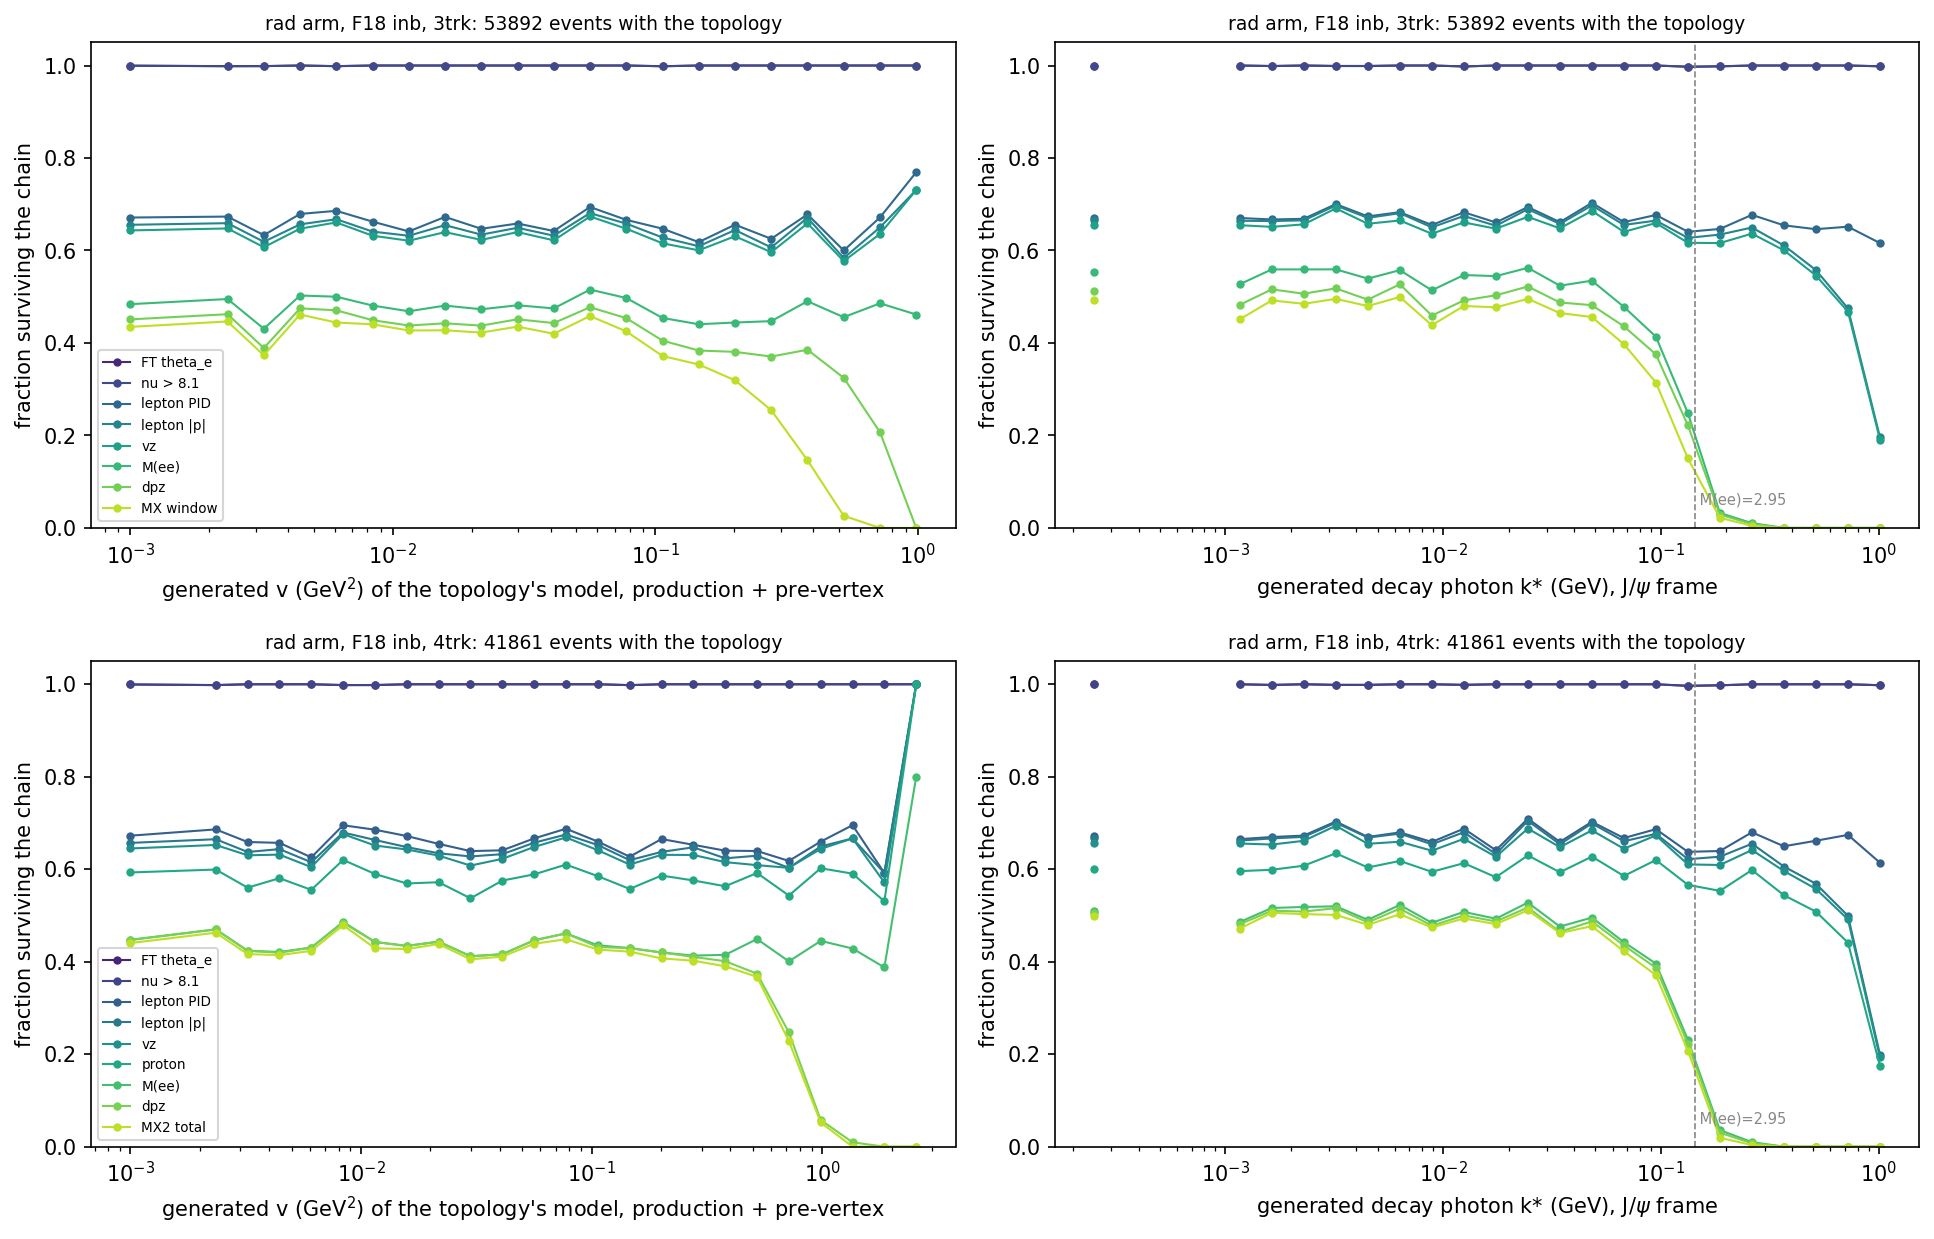
\includegraphics[width=\textwidth]{v1_cuts_vs_radiation.png}
\caption{Survival of the cumulative chain against generated production $v$ (left) and generated decay-photon $k^*$ (right), rad
arm, F18in. The drop from one curve to the next is what that cut removes.}\label{fig:vdist}
\end{figure}

\textbf{Method 2 with the effective cuts} is
$\eta_{\rm int}(v_{50})\,\eta_{\rm ext}(v_{50})\times\hard\times F(K_{50})$. It is still \texttt{rc\_factor} and still uses no Born
MC; the selection enters as its two 50\% points. Against method~1 (Table~\ref{tab:chi2}):
\begin{itemize}
\item $e'e^+e^-p'$: the shape agrees in every binning, both polarities, with $\chi^2$ per cell $\approx1$. Method~1 is
1.1--1.7\% lower throughout: the detector response to radiating leptons (lepton PID alone 0.4--0.9\%, Table~\ref{tab:cutvars}).
\item $e'e^+e^-$: $W$, $Q^2$ and the analysis bins agree in shape. Method~1 is lower by 2\% (inb) and 1\% (outb), the same
detector response. \textbf{Failure in $|t|$} ($\chi^2\approx35/7$), which carries
over into the maps: $-10$ to $-15\%$ at the lowest $|t|$. This is the decay-radiation migration in $t_{e'J/\psi}$ that
the generator-level closure already shows. It is real, and it is not acceptance.

\textbf{This is a finding about M.~Tenorio's analysis, not only a limit of method~2.} In the three-track topology there is no
proton, so any $|t|$ (or $t'$) quoted from $e'e^+e^-$ is built from the lepton pair. Decay radiation moves that $t$:
by $-35$ to $+20\%$ at generator level with no cut, and by $-10$ to $-15\%$ in the lowest $|t|$ bins after the
selection. The analysis note applies one factor, $0.88$, that does not depend on $t$. A $t$-independent decay correction is
wrong in exactly the region that sets the slope. The $W$ and $Q^2$ results of the note are not affected: there, method~2 and the
MC agree. The four-track topology, with $t$ from the proton, is not affected either.
\end{itemize}
\begin{table}[H]\centering\small
\begin{tabular}{llrrrr}\toprule
topology & binning & $\chi^2$/cells inb & mean dev.\ inb & $\chi^2$/cells outb & mean dev.\ outb \\\midrule
$e'e^+e^-$ & W & 9.3/7 & -1.9\% & 11.3/7 & -1.0\% \\
$e'e^+e^-$ & $Q^2$ & 11.2/6 & -2.0\% & 2.5/6 & -0.9\% \\
$e'e^+e^-$ & $|t|$ & 46.7/7 & -2.3\% & 32.4/7 & -1.2\% \\
$e'e^+e^-$ & $(W,|t|)$ at 3 $Q^2$ & 74.2/44 & -2.6\% & 79.8/44 & -1.8\% \\
$e'e^+e^-$ & M.~Tenorio's 3 W bins & 7.3/3 & -2.2\% & 1.1/3 & -0.8\% \\
\midrule
$e'e^+e^-p'$ & W & 5.6/6 & -1.1\% & 4.8/5 & -1.5\% \\
$e'e^+e^-p'$ & $Q^2$ & 7.0/6 & -1.2\% & 3.6/5 & -1.5\% \\
$e'e^+e^-p'$ & $|t|$ & 4.9/7 & -1.1\% & 16.4/6 & -1.7\% \\
$e'e^+e^-p'$ & $(W,|t|)$ at 3 $Q^2$ & 23.8/42 & -1.2\% & 35.8/31 & -1.7\% \\
$e'e^+e^-p'$ & M.~Tenorio's 3 W bins & 1.7/3 & -1.1\% & 3.1/3 & -1.1\% \\
\bottomrule\end{tabular}

\caption{Method 1 against method 2 at effective cuts: $\chi^2$ over cells (statistical error of method 1 only) and the
error-weighted mean deviation.}\label{tab:chi2}
\end{table}

\paragraph{Decomposition} (Fig.~\ref{fig:decomp}). Method 1/method 2 at nominal cuts $-1$, in $W$, split into:
\begin{itemize}
\item the pre-vertex hard part, $-\hardpct\%$;
\item the decay-photon effective edge, $F(K_{50})/F(K)-1$: $-1.8\%$ and $-1.1\%$;
\item the production effective $v$: 0 to $-1\%$;
\item bin migration, method 1 in reconstructed bins against the same events in generated bins: below 1.5\% except at threshold;
\item the residual, the detector's response to radiation beyond those two edges (lepton PID and $|p|$ on radiating
leptons, Table~\ref{tab:cutvars}): about $-1$ to $-2\%$, flat in $W$.
\end{itemize}
Acceptance weighting inside the bin, per-event method~2 against the flat grid, reaches $\pm2\%$ in individual $W$ bins and
$-4\%$ at threshold. It is shown for information. Method~2 is acceptance-weighted per event, so it is not a term of the sum.
The flat average would be wrong by that much.
\begin{figure}[H]\centering
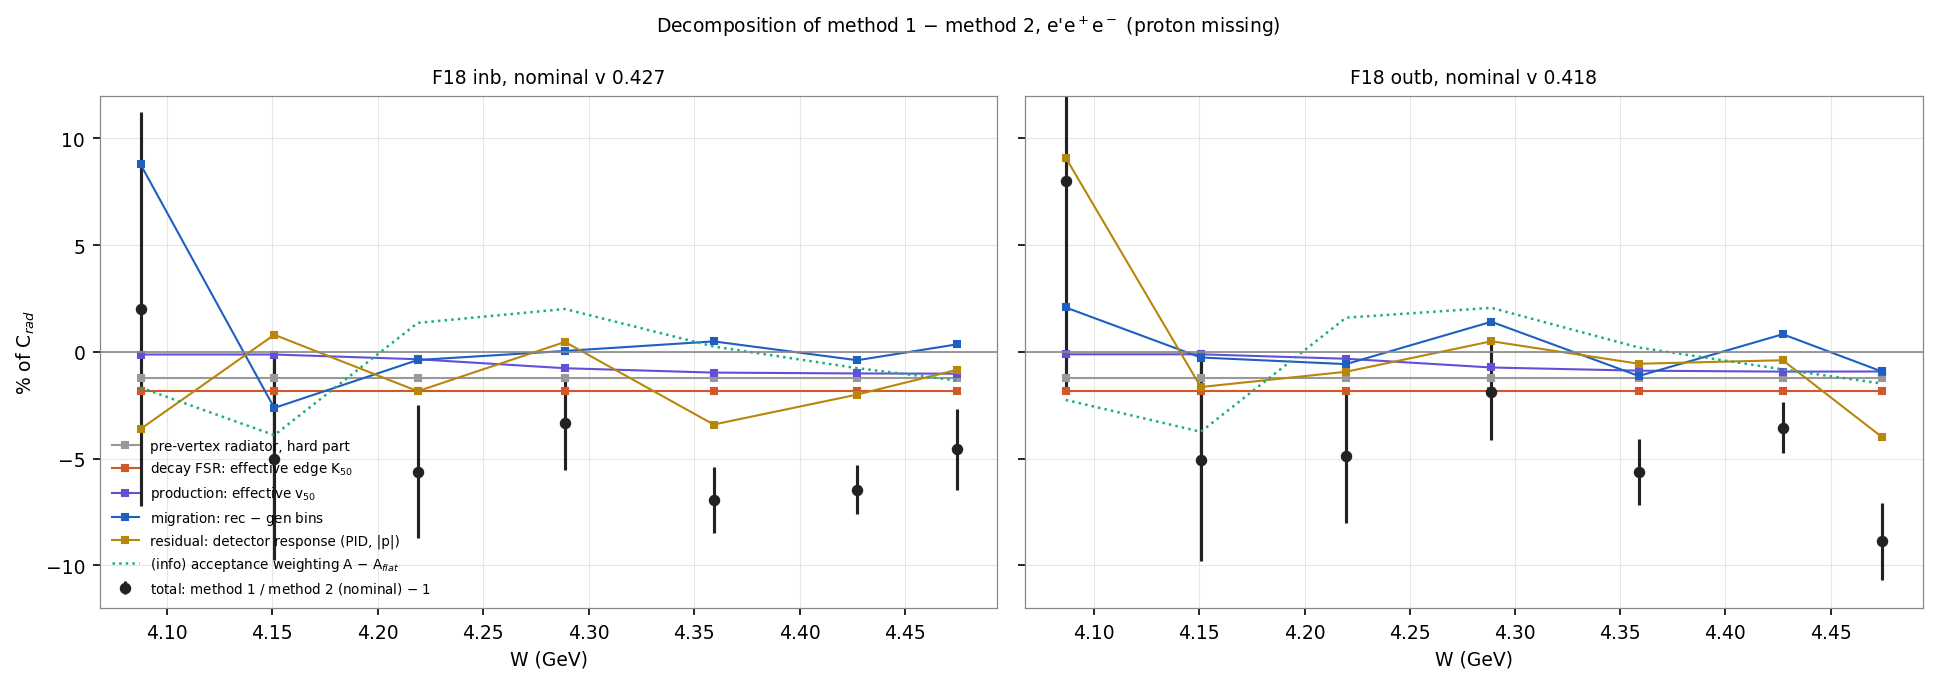
\includegraphics[width=\textwidth]{f4_decomp_3trk.png}
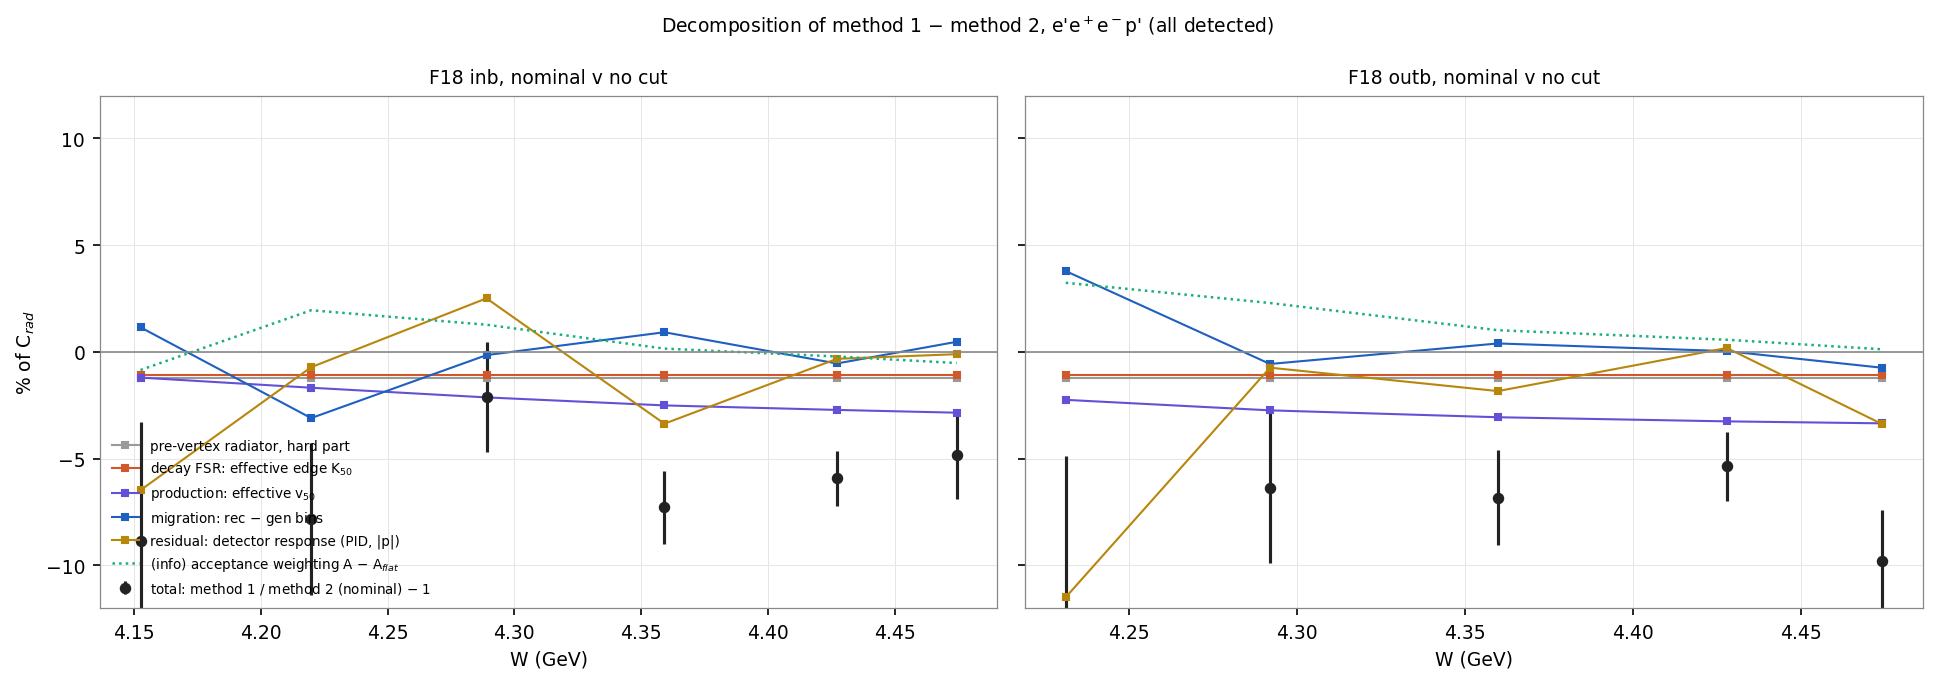
\includegraphics[width=\textwidth]{f4_decomp_4trk.png}
\caption{Decomposition of method 1 $-$ method 2 (nominal cuts) in $W$.}\label{fig:decomp}
\end{figure}

\paragraph{The known generator artefact.} $dN/dE_\gamma$ carries a $\pm8\%$ ripple from the 20-cell majorant grid
(\texttt{generator/tail.py:83}). It is visible in no $\crad$ figure here. The jitter of Fig.~\ref{fig:vdist} is coherent across
curves because they share a denominator; it is statistical, not that ripple.

%=====================================================================
\section{Inbending against outbending}\label{sec:pol}
Method~2 has no torus in it. Any polarity dependence of method~1 is therefore acceptance acting on radiation. Over all cells
of all binnings:
\begin{itemize}
\item three tracks: $\chi^2=\polchiThree/\polnThree$, mean difference $\polmeanThree\%$;
\item four tracks: $\chi^2=\polchiFour/\polnFour$, mean difference $\polmeanFour\%$.
\end{itemize}
In M.~Tenorio's window, three tracks, method 1 is $\BherThreeIn\pm\BherrThreeIn$ (inb) against $\BherThreeOut\pm\BherrThreeOut$ (outb).
\textbf{No polarity dependence is seen at the 1\% level.} Method~1 is radiation, not detector, to that precision.
The parts of it that \emph{are} detector (the effective edges, the PID response) are the same for both torus settings.
\begin{figure}[H]\centering
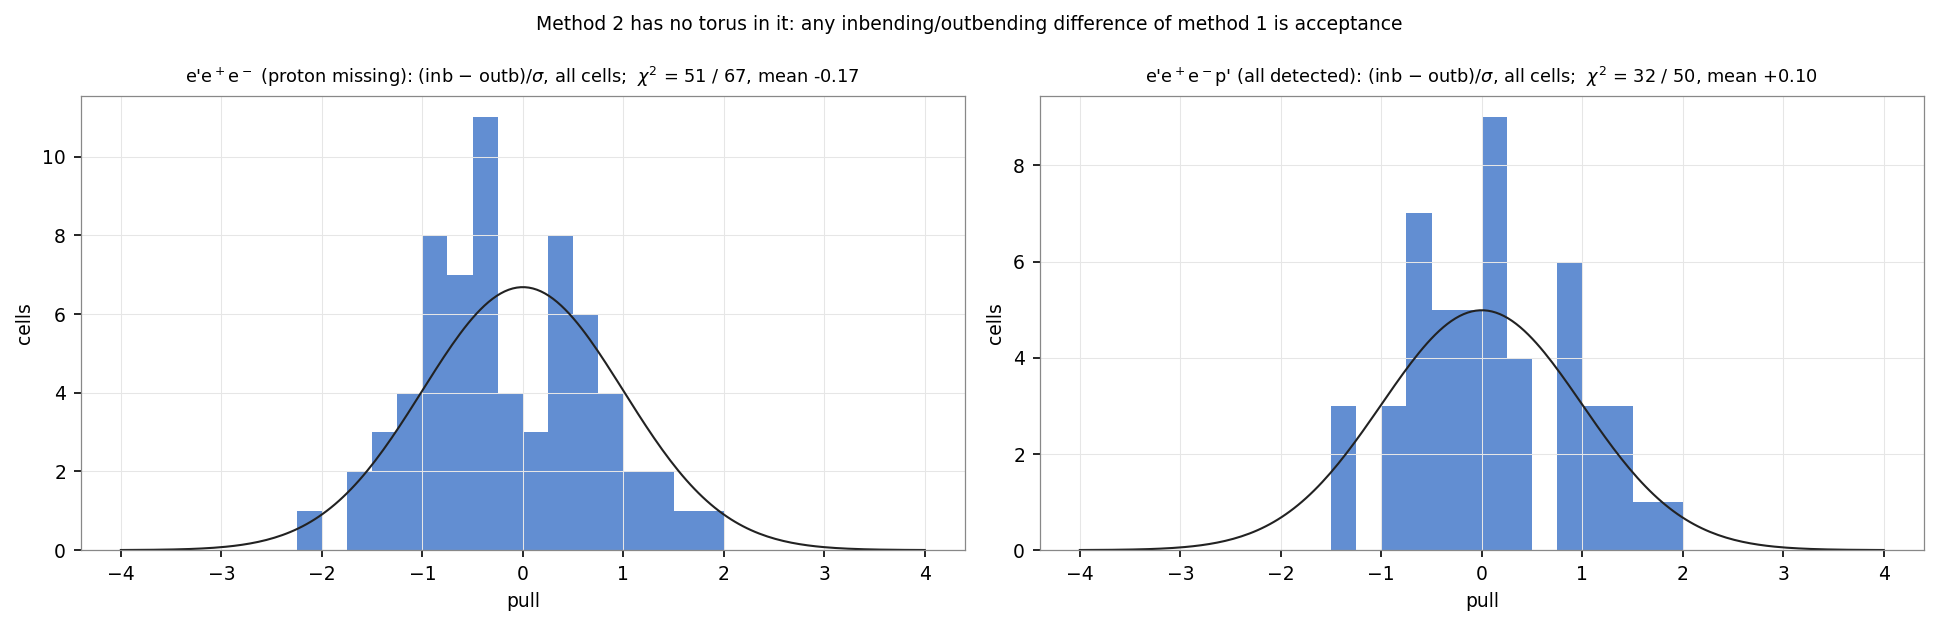
\includegraphics[width=\textwidth]{f5_polarity.png}
\caption{(inb $-$ outb)/$\sigma$ for every cell.}
\end{figure}

%=====================================================================
\section{Against M.~Tenorio's $\crad=0.88\times0.85$}
\begin{itemize}
\item \textbf{Decay radiation.} The note's 0.88 is $F(K)$ at the nominal edge, $\Ffsr$ here. It agrees. The cut the analysis chain really applies is at $K_{50}$, worth
another $-1.1$ to $-1.8\%$ when the yield is counted in the $M(ee)$ window. The fit-based yield of the note includes the radiative
tail in the line shape, so this part applies to the counting method, not to the fit.
\item \textbf{Electron line.} The note's 0.85 at $v_{\max}\approx0.6$. \texttt{rc\_factor} at the actual MX edge, with the pre-vertex
radiator, gives $\prodOne$, $\prodTwo$, $\prodThree$ in the three $W$ bins. The generated 10M gives 0.939 at $v<0.6$. The note's factor is
5--7\% low. That is the largest single difference in this study, and it is in the input to the analysis note, not between our
two methods.
\item \textbf{Total.} Method~1 in the analysis bins is 0.76--0.79 against the note's 0.75. The closeness is a partial cancellation: the
electron-line factor is too low by 5--7\%, and the note omits 3--5\% of selection and detector effects on the decay radiation.
\end{itemize}

%=====================================================================
\section{Conclusions}
\begin{enumerate}
\item The two methods agree in shape once method~2 is told where the selection really cuts: two numbers, $K_{50}$ and
$v_{50}$, read from the MC. With nominal cuts, method~2 is 4--6\% high. The pre-vertex hard part, the decay-photon
effective edge and the production effective $v$ account for 3--4\% of that. The remaining 1--2\% is the detector's
response to radiating leptons. Migration and acceptance weighting are each below 2\%, except at threshold.
\item The one place an analytic correction cannot replace the MC is $|t|$ built from $e'e^+e^-$: decay radiation moves it
by up to 15\% at low $|t|$. For M.~Tenorio's analysis this is an unaccounted $t$-dependent systematic in any three-track $t$
distribution. The single factor 0.88 cannot carry it.
\item The generator's \texttt{sigma\_nb} counts events that the daughter preset then drops. Without correction every
rad/Born normalisation is $\keptpct\%$ high (Sec.~2).
\item Inbending and outbending agree to 1\%.
\item In M.~Tenorio's bins, $\crad=0.76$--$0.79$. The note's decay factor is confirmed; its electron-line factor 0.85 is 5--7\% lower than
\texttt{rc\_factor} at the analysis cut.
\end{enumerate}

\section{What does not reproduce, or is open}
\begin{itemize}
\item Generated decay-photon fraction $\Fgen$ against the formula's $\Ffsr$: explained by the generation preset (Sec.~4).
The fix for \texttt{sigma\_nb} itself belongs in production and has been passed to the Launch generator session.
\item Cuts the ntuple cannot carry (PCAL, BDT, $\chi^2_{\rm PID}$, timing, two-hit FT): they act on the leptons that radiate, as lepton PID does
(0.4--0.9\%). Their effect on $\crad$ is unmeasured.
\item The analysis MX window was fitted on data, ours on Born MC ($\sigma=\mxsig$~GeV). A wider data window moves $v_{50}$; the
three-track $\crad$ depends on it at the $\sim$1\% level (Fig.~\ref{fig:vdist}).
\item Outbending MC at $+1.000$ only (Sec.~2).
\end{itemize}

\section{Reproducibility}
Branch \texttt{jpsi-rc-method-comparison} of \texttt{exclurad\_py}, \texttt{production/analysis/}:
\texttt{rc\_method\_jpsi.py} (reader, selection), \texttt{\_combos.py} (both methods, all binnings),
\texttt{\_closure.py}, \texttt{\_gencuts.py}, \texttt{\_cutvars.py}, \texttt{\_vdist.py}, \texttt{\_plots.py}, \texttt{\_tables.py}.
Data and caches are in \texttt{/Volumes/wd\_14tb/rc\_method\_jpsi}. Every number in this report is in
\texttt{docs/rc\_method\_jpsi/summary.json} and enters the text through \texttt{numbers.tex}.

\appendix
\section{$\crad$ in $(W,|t|)$ at three $Q^2$, and one variable at a time}
The Q$^2$ slices are tertiles, as described in Sec.~5.3. $|t|$ is taken from $e'e^+e^-$ for three tracks and from $p'$ for four tracks.
\begin{table}[H]\centering\footnotesize
\begin{tabular}{lllcccr}\toprule
\multicolumn{7}{l}{$e'e^+e^-$}\\
$Q^2$ (GeV$^2$) & W (GeV) & $|t|$ (GeV$^2$) & inbending & outbending & \textbf{F18 combined} & $n_{\rm rad}$ \\\midrule
0.020--0.027 & 4.15--4.33 & 0.30--1.00 & --- & --- & \textbf{---} & 40 \\
0.020--0.027 & 4.15--4.33 & 1.00--1.36 & --- & --- & \textbf{---} & 72 \\
0.020--0.027 & 4.15--4.33 & 1.36--1.90 & --- & --- & \textbf{---} & 75 \\
0.020--0.027 & 4.15--4.33 & 1.90--5.00 & --- & --- & \textbf{---} & 60 \\
0.020--0.027 & 4.33--4.40 & 0.30--1.00 & 0.785$\pm$0.047 & 0.663$\pm$0.042 & \textbf{0.726$\pm$0.032} & 737 \\
0.020--0.027 & 4.33--4.40 & 1.00--1.36 & 0.762$\pm$0.049 & 0.838$\pm$0.051 & \textbf{0.799$\pm$0.035} & 736 \\
0.020--0.027 & 4.33--4.40 & 1.36--1.90 & 0.875$\pm$0.055 & 0.909$\pm$0.058 & \textbf{0.891$\pm$0.040} & 740 \\
0.020--0.027 & 4.33--4.40 & 1.90--5.00 & 0.871$\pm$0.054 & 0.904$\pm$0.059 & \textbf{0.886$\pm$0.040} & 736 \\
0.020--0.027 & 4.40--4.45 & 0.30--1.00 & 0.741$\pm$0.029 & 0.728$\pm$0.028 & \textbf{0.734$\pm$0.020} & 1862 \\
0.020--0.027 & 4.40--4.45 & 1.00--1.36 & 0.813$\pm$0.038 & 0.884$\pm$0.040 & \textbf{0.847$\pm$0.027} & 1417 \\
0.020--0.027 & 4.40--4.45 & 1.36--1.90 & 0.733$\pm$0.036 & 0.789$\pm$0.038 & \textbf{0.759$\pm$0.026} & 1206 \\
0.020--0.027 & 4.40--4.45 & 1.90--5.00 & 0.768$\pm$0.037 & 0.828$\pm$0.038 & \textbf{0.797$\pm$0.027} & 1306 \\
0.020--0.027 & 4.45--4.60 & 0.30--1.00 & 0.698$\pm$0.027 & 0.730$\pm$0.028 & \textbf{0.714$\pm$0.020} & 1870 \\
0.020--0.027 & 4.45--4.60 & 1.00--1.36 & 0.833$\pm$0.040 & 0.831$\pm$0.040 & \textbf{0.832$\pm$0.028} & 1265 \\
0.020--0.027 & 4.45--4.60 & 1.36--1.90 & 0.785$\pm$0.039 & 0.757$\pm$0.039 & \textbf{0.772$\pm$0.028} & 1117 \\
0.020--0.027 & 4.45--4.60 & 1.90--5.00 & 0.788$\pm$0.039 & 0.759$\pm$0.038 & \textbf{0.774$\pm$0.027} & 1157 \\
\bottomrule\end{tabular}

\medskip

\begin{tabular}{lllcccr}\toprule
\multicolumn{7}{l}{$e'e^+e^-$}\\
$Q^2$ (GeV$^2$) & W (GeV) & $|t|$ (GeV$^2$) & inbending & outbending & \textbf{F18 combined} & $n_{\rm rad}$ \\\midrule
0.027--0.038 & 4.15--4.33 & 0.30--1.00 & 0.715$\pm$0.056 & 0.690$\pm$0.057 & \textbf{0.703$\pm$0.040} & 429 \\
0.027--0.038 & 4.15--4.33 & 1.00--1.36 & 0.777$\pm$0.046 & 0.741$\pm$0.044 & \textbf{0.760$\pm$0.032} & 801 \\
0.027--0.038 & 4.15--4.33 & 1.36--1.90 & 0.779$\pm$0.046 & 0.765$\pm$0.045 & \textbf{0.772$\pm$0.032} & 831 \\
0.027--0.038 & 4.15--4.33 & 1.90--5.00 & 0.836$\pm$0.050 & 0.868$\pm$0.050 & \textbf{0.852$\pm$0.035} & 854 \\
0.027--0.038 & 4.33--4.40 & 0.30--1.00 & 0.652$\pm$0.033 & 0.668$\pm$0.033 & \textbf{0.660$\pm$0.023} & 1122 \\
0.027--0.038 & 4.33--4.40 & 1.00--1.36 & 0.746$\pm$0.036 & 0.751$\pm$0.037 & \textbf{0.749$\pm$0.026} & 1193 \\
0.027--0.038 & 4.33--4.40 & 1.36--1.90 & 0.786$\pm$0.040 & 0.830$\pm$0.042 & \textbf{0.807$\pm$0.029} & 1143 \\
0.027--0.038 & 4.33--4.40 & 1.90--5.00 & 0.769$\pm$0.039 & 0.795$\pm$0.039 & \textbf{0.782$\pm$0.028} & 1159 \\
0.027--0.038 & 4.40--4.45 & 0.30--1.00 & 0.647$\pm$0.028 & 0.704$\pm$0.031 & \textbf{0.674$\pm$0.021} & 1443 \\
0.027--0.038 & 4.40--4.45 & 1.00--1.36 & 0.855$\pm$0.041 & 0.831$\pm$0.041 & \textbf{0.843$\pm$0.029} & 1253 \\
0.027--0.038 & 4.40--4.45 & 1.36--1.90 & 0.822$\pm$0.042 & 0.806$\pm$0.041 & \textbf{0.814$\pm$0.029} & 1116 \\
0.027--0.038 & 4.40--4.45 & 1.90--5.00 & 0.760$\pm$0.039 & 0.884$\pm$0.044 & \textbf{0.818$\pm$0.029} & 1146 \\
0.027--0.038 & 4.45--4.60 & 0.30--1.00 & 0.746$\pm$0.038 & 0.693$\pm$0.036 & \textbf{0.720$\pm$0.026} & 1051 \\
0.027--0.038 & 4.45--4.60 & 1.00--1.36 & 0.808$\pm$0.053 & 0.755$\pm$0.050 & \textbf{0.782$\pm$0.037} & 653 \\
0.027--0.038 & 4.45--4.60 & 1.36--1.90 & 0.778$\pm$0.054 & 0.795$\pm$0.055 & \textbf{0.786$\pm$0.039} & 600 \\
0.027--0.038 & 4.45--4.60 & 1.90--5.00 & 0.760$\pm$0.051 & 0.697$\pm$0.049 & \textbf{0.731$\pm$0.036} & 591 \\
\bottomrule\end{tabular}

\medskip

\begin{tabular}{lllcccr}\toprule
\multicolumn{7}{l}{$e'e^+e^-$}\\
$Q^2$ (GeV$^2$) & W (GeV) & $|t|$ (GeV$^2$) & inbending & outbending & \textbf{F18 combined} & $n_{\rm rad}$ \\\midrule
0.038--0.120 & 4.15--4.33 & 0.30--1.00 & 0.692$\pm$0.042 & 0.634$\pm$0.039 & \textbf{0.664$\pm$0.028} & 750 \\
0.038--0.120 & 4.15--4.33 & 1.00--1.36 & 0.743$\pm$0.030 & 0.689$\pm$0.027 & \textbf{0.716$\pm$0.020} & 1736 \\
0.038--0.120 & 4.15--4.33 & 1.36--1.90 & 0.776$\pm$0.029 & 0.844$\pm$0.031 & \textbf{0.809$\pm$0.021} & 2104 \\
0.038--0.120 & 4.15--4.33 & 1.90--5.00 & 0.767$\pm$0.029 & 0.819$\pm$0.031 & \textbf{0.791$\pm$0.021} & 2066 \\
0.038--0.120 & 4.33--4.40 & 0.30--1.00 & 0.645$\pm$0.035 & 0.679$\pm$0.036 & \textbf{0.662$\pm$0.025} & 957 \\
0.038--0.120 & 4.33--4.40 & 1.00--1.36 & 0.793$\pm$0.042 & 0.826$\pm$0.042 & \textbf{0.809$\pm$0.030} & 1078 \\
0.038--0.120 & 4.33--4.40 & 1.36--1.90 & 0.802$\pm$0.043 & 0.747$\pm$0.041 & \textbf{0.775$\pm$0.030} & 978 \\
0.038--0.120 & 4.33--4.40 & 1.90--5.00 & 0.757$\pm$0.041 & 0.810$\pm$0.043 & \textbf{0.782$\pm$0.030} & 1015 \\
0.038--0.120 & 4.40--4.45 & 0.30--1.00 & 0.680$\pm$0.041 & 0.701$\pm$0.043 & \textbf{0.690$\pm$0.030} & 759 \\
0.038--0.120 & 4.40--4.45 & 1.00--1.36 & 0.824$\pm$0.054 & 0.755$\pm$0.051 & \textbf{0.791$\pm$0.037} & 645 \\
0.038--0.120 & 4.40--4.45 & 1.36--1.90 & 0.890$\pm$0.060 & 0.849$\pm$0.063 & \textbf{0.872$\pm$0.044} & 599 \\
0.038--0.120 & 4.40--4.45 & 1.90--5.00 & 0.777$\pm$0.053 & 0.805$\pm$0.056 & \textbf{0.790$\pm$0.038} & 611 \\
0.038--0.120 & 4.45--4.60 & 0.30--1.00 & 0.741$\pm$0.070 & 0.682$\pm$0.065 & \textbf{0.712$\pm$0.048} & 310 \\
0.038--0.120 & 4.45--4.60 & 1.00--1.36 & \textit{0.864$\pm$0.100} & \textit{0.731$\pm$0.084} & \textbf{0.796$\pm$0.065} & 219 \\
0.038--0.120 & 4.45--4.60 & 1.36--1.90 & \textit{1.128$\pm$0.129} & \textit{0.879$\pm$0.106} & \textbf{1.006$\pm$0.084} & 227 \\
0.038--0.120 & 4.45--4.60 & 1.90--5.00 & \textit{0.866$\pm$0.101} & \textit{0.808$\pm$0.096} & \textbf{0.838$\pm$0.070} & 213 \\
\bottomrule\end{tabular}

\medskip


\caption{$\crad(W,|t|)$, $e'e^+e^-$.}
\end{table}
\begin{table}[H]\centering\footnotesize
\begin{tabular}{lllcccr}\toprule
\multicolumn{7}{l}{$e'e^+e^-p'$}\\
$Q^2$ (GeV$^2$) & W (GeV) & $|t|$ (GeV$^2$) & inbending & outbending & \textbf{F18 combined} & $n_{\rm rad}$ \\\midrule
0.020--0.027 & 4.15--4.33 & 0.30--1.00 & --- & --- & \textbf{---} & 20 \\
0.020--0.027 & 4.15--4.33 & 1.00--1.36 & --- & --- & \textbf{---} & 29 \\
0.020--0.027 & 4.15--4.33 & 1.36--1.90 & --- & --- & \textbf{---} & 50 \\
0.020--0.027 & 4.15--4.33 & 1.90--5.00 & --- & --- & \textbf{---} & 44 \\
0.020--0.027 & 4.33--4.40 & 0.30--1.00 & 0.743$\pm$0.049 & --- & \textbf{0.743$\pm$0.049$^\dagger$} & 332 \\
0.020--0.027 & 4.33--4.40 & 1.00--1.36 & 0.846$\pm$0.062 & 0.836$\pm$0.069 & \textbf{0.841$\pm$0.046} & 490 \\
0.020--0.027 & 4.33--4.40 & 1.36--1.90 & 0.780$\pm$0.062 & 0.845$\pm$0.069 & \textbf{0.809$\pm$0.046} & 453 \\
0.020--0.027 & 4.33--4.40 & 1.90--5.00 & 0.850$\pm$0.056 & 0.916$\pm$0.065 & \textbf{0.878$\pm$0.042} & 644 \\
0.020--0.027 & 4.40--4.45 & 0.30--1.00 & 0.802$\pm$0.034 & \textit{0.774$\pm$0.084} & \textbf{0.798$\pm$0.031} & 931 \\
0.020--0.027 & 4.40--4.45 & 1.00--1.36 & 0.776$\pm$0.042 & 0.787$\pm$0.046 & \textbf{0.781$\pm$0.031} & 913 \\
0.020--0.027 & 4.40--4.45 & 1.36--1.90 & 0.791$\pm$0.046 & 0.797$\pm$0.047 & \textbf{0.794$\pm$0.033} & 849 \\
0.020--0.027 & 4.40--4.45 & 1.90--5.00 & 0.748$\pm$0.038 & 0.822$\pm$0.041 & \textbf{0.783$\pm$0.028} & 1135 \\
0.020--0.027 & 4.45--4.60 & 0.30--1.00 & 0.763$\pm$0.032 & 0.768$\pm$0.062 & \textbf{0.764$\pm$0.029} & 1015 \\
0.020--0.027 & 4.45--4.60 & 1.00--1.36 & 0.796$\pm$0.045 & 0.784$\pm$0.047 & \textbf{0.791$\pm$0.033} & 855 \\
0.020--0.027 & 4.45--4.60 & 1.36--1.90 & 0.788$\pm$0.045 & 0.826$\pm$0.050 & \textbf{0.805$\pm$0.033} & 842 \\
0.020--0.027 & 4.45--4.60 & 1.90--5.00 & 0.827$\pm$0.043 & 0.775$\pm$0.041 & \textbf{0.802$\pm$0.030} & 1048 \\
\bottomrule\end{tabular}

\medskip

\begin{tabular}{lllcccr}\toprule
\multicolumn{7}{l}{$e'e^+e^-p'$}\\
$Q^2$ (GeV$^2$) & W (GeV) & $|t|$ (GeV$^2$) & inbending & outbending & \textbf{F18 combined} & $n_{\rm rad}$ \\\midrule
0.027--0.038 & 4.15--4.33 & 0.30--1.00 & 0.761$\pm$0.065 & --- & \textbf{0.761$\pm$0.065$^\dagger$} & 195 \\
0.027--0.038 & 4.15--4.33 & 1.00--1.36 & 0.800$\pm$0.056 & --- & \textbf{0.800$\pm$0.056$^\dagger$} & 347 \\
0.027--0.038 & 4.15--4.33 & 1.36--1.90 & 0.782$\pm$0.056 & 0.668$\pm$0.058 & \textbf{0.735$\pm$0.041} & 461 \\
0.027--0.038 & 4.15--4.33 & 1.90--5.00 & 0.821$\pm$0.054 & 0.811$\pm$0.060 & \textbf{0.816$\pm$0.040} & 603 \\
0.027--0.038 & 4.33--4.40 & 0.30--1.00 & 0.725$\pm$0.038 & --- & \textbf{0.725$\pm$0.038$^\dagger$} & 513 \\
0.027--0.038 & 4.33--4.40 & 1.00--1.36 & 0.712$\pm$0.042 & 0.744$\pm$0.050 & \textbf{0.725$\pm$0.032} & 714 \\
0.027--0.038 & 4.33--4.40 & 1.36--1.90 & 0.794$\pm$0.048 & 0.776$\pm$0.049 & \textbf{0.786$\pm$0.034} & 761 \\
0.027--0.038 & 4.33--4.40 & 1.90--5.00 & 0.761$\pm$0.040 & 0.757$\pm$0.042 & \textbf{0.759$\pm$0.029} & 971 \\
0.027--0.038 & 4.40--4.45 & 0.30--1.00 & 0.793$\pm$0.037 & --- & \textbf{0.793$\pm$0.037$^\dagger$} & 763 \\
0.027--0.038 & 4.40--4.45 & 1.00--1.36 & 0.807$\pm$0.046 & 0.857$\pm$0.051 & \textbf{0.829$\pm$0.034} & 857 \\
0.027--0.038 & 4.40--4.45 & 1.36--1.90 & 0.798$\pm$0.049 & 0.731$\pm$0.047 & \textbf{0.766$\pm$0.034} & 736 \\
0.027--0.038 & 4.40--4.45 & 1.90--5.00 & 0.766$\pm$0.042 & 0.847$\pm$0.046 & \textbf{0.803$\pm$0.031} & 978 \\
0.027--0.038 & 4.45--4.60 & 0.30--1.00 & 0.812$\pm$0.045 & \textit{0.725$\pm$0.081} & \textbf{0.795$\pm$0.040} & 578 \\
0.027--0.038 & 4.45--4.60 & 1.00--1.36 & 0.804$\pm$0.064 & 0.722$\pm$0.059 & \textbf{0.765$\pm$0.044} & 439 \\
0.027--0.038 & 4.45--4.60 & 1.36--1.90 & 0.770$\pm$0.063 & 0.771$\pm$0.065 & \textbf{0.770$\pm$0.045} & 416 \\
0.027--0.038 & 4.45--4.60 & 1.90--5.00 & 0.717$\pm$0.051 & 0.712$\pm$0.052 & \textbf{0.715$\pm$0.037} & 535 \\
\bottomrule\end{tabular}

\medskip

\begin{tabular}{lllcccr}\toprule
\multicolumn{7}{l}{$e'e^+e^-p'$}\\
$Q^2$ (GeV$^2$) & W (GeV) & $|t|$ (GeV$^2$) & inbending & outbending & \textbf{F18 combined} & $n_{\rm rad}$ \\\midrule
0.038--0.120 & 4.15--4.33 & 0.30--1.00 & 0.775$\pm$0.050 & --- & \textbf{0.775$\pm$0.050$^\dagger$} & 343 \\
0.038--0.120 & 4.15--4.33 & 1.00--1.36 & 0.760$\pm$0.036 & --- & \textbf{0.760$\pm$0.036$^\dagger$} & 703 \\
0.038--0.120 & 4.15--4.33 & 1.36--1.90 & 0.753$\pm$0.035 & 0.746$\pm$0.048 & \textbf{0.751$\pm$0.029} & 981 \\
0.038--0.120 & 4.15--4.33 & 1.90--5.00 & 0.783$\pm$0.033 & 0.813$\pm$0.044 & \textbf{0.794$\pm$0.026} & 1324 \\
0.038--0.120 & 4.33--4.40 & 0.30--1.00 & 0.751$\pm$0.042 & --- & \textbf{0.751$\pm$0.042$^\dagger$} & 452 \\
0.038--0.120 & 4.33--4.40 & 1.00--1.36 & 0.807$\pm$0.051 & 0.690$\pm$0.054 & \textbf{0.761$\pm$0.037} & 591 \\
0.038--0.120 & 4.33--4.40 & 1.36--1.90 & 0.787$\pm$0.052 & 0.660$\pm$0.046 & \textbf{0.727$\pm$0.035} & 616 \\
0.038--0.120 & 4.33--4.40 & 1.90--5.00 & 0.745$\pm$0.043 & 0.796$\pm$0.047 & \textbf{0.769$\pm$0.032} & 847 \\
0.038--0.120 & 4.40--4.45 & 0.30--1.00 & 0.799$\pm$0.051 & --- & \textbf{0.799$\pm$0.051$^\dagger$} & 401 \\
0.038--0.120 & 4.40--4.45 & 1.00--1.36 & 0.809$\pm$0.063 & 0.837$\pm$0.072 & \textbf{0.821$\pm$0.048} & 436 \\
0.038--0.120 & 4.40--4.45 & 1.36--1.90 & 0.784$\pm$0.066 & 0.868$\pm$0.078 & \textbf{0.820$\pm$0.051} & 386 \\
0.038--0.120 & 4.40--4.45 & 1.90--5.00 & 0.777$\pm$0.055 & 0.759$\pm$0.057 & \textbf{0.769$\pm$0.040} & 538 \\
0.038--0.120 & 4.45--4.60 & 0.30--1.00 & \textit{0.793$\pm$0.079} & --- & \textbf{\textit{0.793$\pm$0.079}$^\dagger$} & 166 \\
0.038--0.120 & 4.45--4.60 & 1.00--1.36 & --- & --- & \textbf{---} & 149 \\
0.038--0.120 & 4.45--4.60 & 1.36--1.90 & \textit{1.120$\pm$0.141} & --- & \textbf{\textit{1.120$\pm$0.141}$^\dagger$} & 181 \\
0.038--0.120 & 4.45--4.60 & 1.90--5.00 & --- & --- & \textbf{---} & 189 \\
\bottomrule\end{tabular}

\medskip


\caption{$\crad(W,|t|)$, $e'e^+e^-p'$.}
\end{table}
\begin{table}[H]\centering\footnotesize
\begin{tabular}{lcccr}\toprule
\multicolumn{5}{l}{$e'e^+e^-$}\\
W (GeV) & inbending & outbending & \textbf{F18 combined} & $n_{\rm rad}$ \\\midrule
4.04--4.11 & 0.762$\pm$0.069 & 0.803$\pm$0.072 & \textbf{0.782$\pm$0.050} & 357 \\
4.11--4.18 & 0.739$\pm$0.037 & 0.739$\pm$0.037 & \textbf{0.739$\pm$0.026} & 1144 \\
4.18--4.25 & 0.752$\pm$0.025 & 0.760$\pm$0.025 & \textbf{0.756$\pm$0.018} & 2628 \\
4.25--4.32 & 0.781$\pm$0.018 & 0.792$\pm$0.018 & \textbf{0.786$\pm$0.013} & 5500 \\
4.32--4.39 & 0.757$\pm$0.013 & 0.767$\pm$0.013 & \textbf{0.761$\pm$0.009} & 10507 \\
4.39--4.46 & 0.763$\pm$0.009 & 0.786$\pm$0.010 & \textbf{0.774$\pm$0.007} & 18954 \\
4.46--4.53 & 0.780$\pm$0.015 & 0.744$\pm$0.015 & \textbf{0.763$\pm$0.011} & 7278 \\
4.53--4.60 & --- & --- & \textbf{---} & 0 \\
\bottomrule\end{tabular}

\medskip

\begin{tabular}{lcccr}\toprule
\multicolumn{5}{l}{$e'e^+e^-$}\\
$Q^2$ (GeV$^2$) & inbending & outbending & \textbf{F18 combined} & $n_{\rm rad}$ \\\midrule
0.001--0.020 & 0.762$\pm$0.034 & 0.757$\pm$0.034 & \textbf{0.759$\pm$0.024} & 1427 \\
0.020--0.035 & 0.766$\pm$0.008 & 0.777$\pm$0.008 & \textbf{0.771$\pm$0.006} & 26572 \\
0.035--0.050 & 0.781$\pm$0.012 & 0.772$\pm$0.012 & \textbf{0.777$\pm$0.009} & 11513 \\
0.050--0.070 & 0.736$\pm$0.018 & 0.759$\pm$0.018 & \textbf{0.747$\pm$0.013} & 4932 \\
0.070--0.090 & 0.720$\pm$0.034 & 0.768$\pm$0.035 & \textbf{0.743$\pm$0.024} & 1336 \\
0.090--0.110 & 0.767$\pm$0.063 & 0.794$\pm$0.064 & \textbf{0.780$\pm$0.045} & 437 \\
0.110--0.143 & --- & --- & \textbf{---} & 151 \\
\bottomrule\end{tabular}

\medskip

\begin{tabular}{lcccr}\toprule
\multicolumn{5}{l}{$e'e^+e^-$}\\
$|t|$ (GeV$^2$) & inbending & outbending & \textbf{F18 combined} & $n_{\rm rad}$ \\\midrule
0.3--0.5 & --- & --- & \textbf{---} & 124 \\
0.5--0.7 & 0.615$\pm$0.022 & 0.636$\pm$0.022 & \textbf{0.625$\pm$0.015} & 2212 \\
0.7--0.9 & 0.694$\pm$0.015 & 0.708$\pm$0.015 & \textbf{0.701$\pm$0.011} & 5972 \\
0.9--1.2 & 0.777$\pm$0.013 & 0.765$\pm$0.013 & \textbf{0.771$\pm$0.009} & 10284 \\
1.2--1.6 & 0.809$\pm$0.013 & 0.804$\pm$0.013 & \textbf{0.807$\pm$0.009} & 10587 \\
1.6--2.2 & 0.787$\pm$0.014 & 0.813$\pm$0.014 & \textbf{0.799$\pm$0.010} & 9483 \\
2.2--3.0 & 0.778$\pm$0.017 & 0.802$\pm$0.017 & \textbf{0.789$\pm$0.012} & 6131 \\
3.0--5.0 & 0.798$\pm$0.034 & 0.821$\pm$0.035 & \textbf{0.809$\pm$0.025} & 1575 \\
\bottomrule\end{tabular}

\medskip


\caption{$\crad$ in one variable, the other two integrated over the box ($W$ 4.04--4.60, $Q^2$ 0.001--0.143, $|t|$ 0.3--5.0), $e'e^+e^-$.}
\end{table}
\begin{table}[H]\centering\footnotesize
\begin{tabular}{lcccr}\toprule
\multicolumn{5}{l}{$e'e^+e^-p'$}\\
W (GeV) & inbending & outbending & \textbf{F18 combined} & $n_{\rm rad}$ \\\midrule
4.04--4.11 & --- & --- & \textbf{---} & 69 \\
4.11--4.18 & 0.718$\pm$0.044 & --- & \textbf{0.718$\pm$0.044$^\dagger$} & 375 \\
4.18--4.25 & 0.743$\pm$0.029 & 0.716$\pm$0.060 & \textbf{0.738$\pm$0.026} & 1137 \\
4.25--4.32 & 0.800$\pm$0.021 & 0.773$\pm$0.029 & \textbf{0.792$\pm$0.017} & 3083 \\
4.32--4.39 & 0.766$\pm$0.014 & 0.777$\pm$0.019 & \textbf{0.770$\pm$0.011} & 6649 \\
4.39--4.46 & 0.784$\pm$0.011 & 0.795$\pm$0.013 & \textbf{0.788$\pm$0.008} & 12656 \\
4.46--4.53 & 0.798$\pm$0.017 & 0.761$\pm$0.020 & \textbf{0.783$\pm$0.013} & 5042 \\
4.53--4.60 & --- & --- & \textbf{---} & 0 \\
\bottomrule\end{tabular}

\medskip

\begin{tabular}{lcccr}\toprule
\multicolumn{5}{l}{$e'e^+e^-p'$}\\
$Q^2$ (GeV$^2$) & inbending & outbending & \textbf{F18 combined} & $n_{\rm rad}$ \\\midrule
0.001--0.020 & 0.760$\pm$0.038 & 0.744$\pm$0.045 & \textbf{0.753$\pm$0.029} & 960 \\
0.020--0.035 & 0.782$\pm$0.009 & 0.789$\pm$0.011 & \textbf{0.785$\pm$0.007} & 17552 \\
0.035--0.050 & 0.798$\pm$0.014 & 0.773$\pm$0.019 & \textbf{0.789$\pm$0.011} & 6969 \\
0.050--0.070 & 0.745$\pm$0.021 & 0.767$\pm$0.031 & \textbf{0.752$\pm$0.017} & 2689 \\
0.070--0.090 & 0.736$\pm$0.041 & 0.722$\pm$0.066 & \textbf{0.732$\pm$0.035} & 627 \\
0.090--0.110 & 0.710$\pm$0.071 & --- & \textbf{0.710$\pm$0.071$^\dagger$} & 164 \\
0.110--0.143 & --- & --- & \textbf{---} & 50 \\
\bottomrule\end{tabular}

\medskip

\begin{tabular}{lcccr}\toprule
\multicolumn{5}{l}{$e'e^+e^-p'$}\\
$|t|$ (GeV$^2$) & inbending & outbending & \textbf{F18 combined} & $n_{\rm rad}$ \\\midrule
0.3--0.5 & --- & --- & \textbf{---} & 11 \\
0.5--0.7 & 0.751$\pm$0.025 & --- & \textbf{0.751$\pm$0.025$^\dagger$} & 1235 \\
0.7--0.9 & 0.773$\pm$0.018 & 0.680$\pm$0.063 & \textbf{0.768$\pm$0.017} & 2855 \\
0.9--1.2 & 0.791$\pm$0.015 & 0.763$\pm$0.021 & \textbf{0.782$\pm$0.012} & 5744 \\
1.2--1.6 & 0.788$\pm$0.016 & 0.762$\pm$0.017 & \textbf{0.777$\pm$0.012} & 6449 \\
1.6--2.2 & 0.782$\pm$0.017 & 0.819$\pm$0.019 & \textbf{0.798$\pm$0.012} & 6073 \\
2.2--3.0 & 0.755$\pm$0.020 & 0.751$\pm$0.021 & \textbf{0.753$\pm$0.015} & 3845 \\
3.0--5.0 & 0.798$\pm$0.025 & 0.824$\pm$0.028 & \textbf{0.809$\pm$0.018} & 2799 \\
\bottomrule\end{tabular}

\medskip


\caption{As above, $e'e^+e^-p'$.}
\end{table}
\end{document}
